\documentclass[twoside]{book}

% Packages required by doxygen
\usepackage{fixltx2e}
\usepackage{calc}
\usepackage{doxygen}
\usepackage[export]{adjustbox} % also loads graphicx
\usepackage{graphicx}
\usepackage[utf8]{inputenc}
\usepackage{makeidx}
\usepackage{multicol}
\usepackage{multirow}
\PassOptionsToPackage{warn}{textcomp}
\usepackage{textcomp}
\usepackage[nointegrals]{wasysym}
\usepackage[table]{xcolor}

% Font selection
\usepackage[T1]{fontenc}
\usepackage[scaled=.90]{helvet}
\usepackage{courier}
\usepackage{amssymb}
\usepackage{sectsty}
\renewcommand{\familydefault}{\sfdefault}
\allsectionsfont{%
  \fontseries{bc}\selectfont%
  \color{darkgray}%
}
\renewcommand{\DoxyLabelFont}{%
  \fontseries{bc}\selectfont%
  \color{darkgray}%
}
\newcommand{\+}{\discretionary{\mbox{\scriptsize$\hookleftarrow$}}{}{}}

% Page & text layout
\usepackage{geometry}
\geometry{%
  a4paper,%
  top=2.5cm,%
  bottom=2.5cm,%
  left=2.5cm,%
  right=2.5cm%
}
\tolerance=750
\hfuzz=15pt
\hbadness=750
\setlength{\emergencystretch}{15pt}
\setlength{\parindent}{0cm}
\setlength{\parskip}{3ex plus 2ex minus 2ex}
\makeatletter
\renewcommand{\paragraph}{%
  \@startsection{paragraph}{4}{0ex}{-1.0ex}{1.0ex}{%
    \normalfont\normalsize\bfseries\SS@parafont%
  }%
}
\renewcommand{\subparagraph}{%
  \@startsection{subparagraph}{5}{0ex}{-1.0ex}{1.0ex}{%
    \normalfont\normalsize\bfseries\SS@subparafont%
  }%
}
\makeatother

% Headers & footers
\usepackage{fancyhdr}
\pagestyle{fancyplain}
\fancyhead[LE]{\fancyplain{}{\bfseries\thepage}}
\fancyhead[CE]{\fancyplain{}{}}
\fancyhead[RE]{\fancyplain{}{\bfseries\leftmark}}
\fancyhead[LO]{\fancyplain{}{\bfseries\rightmark}}
\fancyhead[CO]{\fancyplain{}{}}
\fancyhead[RO]{\fancyplain{}{\bfseries\thepage}}
\fancyfoot[LE]{\fancyplain{}{}}
\fancyfoot[CE]{\fancyplain{}{}}
\fancyfoot[RE]{\fancyplain{}{\bfseries\scriptsize Generated by Doxygen }}
\fancyfoot[LO]{\fancyplain{}{\bfseries\scriptsize Generated by Doxygen }}
\fancyfoot[CO]{\fancyplain{}{}}
\fancyfoot[RO]{\fancyplain{}{}}
\renewcommand{\footrulewidth}{0.4pt}
\renewcommand{\chaptermark}[1]{%
  \markboth{#1}{}%
}
\renewcommand{\sectionmark}[1]{%
  \markright{\thesection\ #1}%
}

% Indices & bibliography
\usepackage{natbib}
\usepackage[titles]{tocloft}
\setcounter{tocdepth}{3}
\setcounter{secnumdepth}{5}
\makeindex

% Hyperlinks (required, but should be loaded last)
\usepackage{ifpdf}
\ifpdf
  \usepackage[pdftex,pagebackref=true]{hyperref}
\else
  \usepackage[ps2pdf,pagebackref=true]{hyperref}
\fi
\hypersetup{%
  colorlinks=true,%
  linkcolor=blue,%
  citecolor=blue,%
  unicode%
}

% Custom commands
\newcommand{\clearemptydoublepage}{%
  \newpage{\pagestyle{empty}\cleardoublepage}%
}

\usepackage{caption}
\captionsetup{labelsep=space,justification=centering,font={bf},singlelinecheck=off,skip=4pt,position=top}

%===== C O N T E N T S =====

\begin{document}

% Titlepage & ToC
\hypersetup{pageanchor=false,
             bookmarksnumbered=true,
             pdfencoding=unicode
            }
\pagenumbering{roman}
\begin{titlepage}
\vspace*{7cm}
\begin{center}%
{\Large Jogo da velha }\\
\vspace*{1cm}
{\large Generated by Doxygen 1.8.11}\\
\end{center}
\end{titlepage}
\clearemptydoublepage
\tableofcontents
\clearemptydoublepage
\pagenumbering{arabic}
\hypersetup{pageanchor=true}

%--- Begin generated contents ---
\chapter{Main Page}
\label{index}\hypertarget{index}{}Código fonte do jogo da velha. 

Esse código, juntamente com a Main, representa uma série de funções que controlam o jogo da velha!

\begin{DoxyAuthor}{Author}
Lucas Ribeiro 
\end{DoxyAuthor}
\begin{DoxyDate}{Date}
25/05/2017 
\end{DoxyDate}

\chapter{R\+E\+A\+D\+ME}
\label{md_README}
\hypertarget{md_README}{}
Jogo da Velha I.\+A 
\chapter{Data Structure Index}
\section{Data Structures}
Here are the data structures with brief descriptions\+:\begin{DoxyCompactList}
\item\contentsline{section}{\hyperlink{structnode}{node} }{\pageref{structnode}}{}
\item\contentsline{section}{\hyperlink{structstruct}{struct} \\*Essa estrutura representa um nó que irá formar a árvore A\+VL }{\pageref{structstruct}}{}
\end{DoxyCompactList}

\chapter{File Index}
\section{File List}
Here is a list of all documented files with brief descriptions\+:\begin{DoxyCompactList}
\item\contentsline{section}{\hyperlink{avl__jogo__da__velha_8c}{avl\+\_\+jogo\+\_\+da\+\_\+velha.\+c} \\*Implementação das funções descritas na biblioteca \hyperlink{avl__jogo__da__velha_8h}{avl\+\_\+jogo\+\_\+da\+\_\+velha.\+h} }{\pageref{avl__jogo__da__velha_8c}}{}
\item\contentsline{section}{\hyperlink{avl__jogo__da__velha_8h}{avl\+\_\+jogo\+\_\+da\+\_\+velha.\+h} \\*É uma biblioteca para manipulação de A\+VL }{\pageref{avl__jogo__da__velha_8h}}{}
\item\contentsline{section}{\hyperlink{jogo__da__velha__main_8c}{jogo\+\_\+da\+\_\+velha\+\_\+main.\+c} \\*Código fonte do jogo da velha }{\pageref{jogo__da__velha__main_8c}}{}
\end{DoxyCompactList}

\chapter{Data Structure Documentation}
\hypertarget{structnode}{}\section{node Struct Reference}
\label{structnode}\index{node@{node}}


Collaboration diagram for node\+:\nopagebreak
\begin{figure}[H]
\begin{center}
\leavevmode
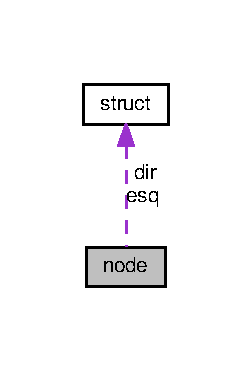
\includegraphics[width=121pt]{structnode__coll__graph}
\end{center}
\end{figure}
\subsection*{Data Fields}
\begin{DoxyCompactItemize}
\item 
int \hyperlink{structnode_a4a9a339d4d22e3b9e5fd31964220a195}{chave}
\item 
int \hyperlink{structnode_adff0ea2ada1722208aa1c811d1019d39}{jogador}
\item 
int \hyperlink{structnode_a778b6b04a3f5e4401e90b192cb05b557}{altura}
\item 
\hyperlink{structstruct}{struct} \hyperlink{structnode}{node} $\ast$ \hyperlink{structnode_a2d0c3d7f54adedaa369899f4df5a4b6a}{esq}
\item 
\hyperlink{structstruct}{struct} \hyperlink{structnode}{node} $\ast$ \hyperlink{structnode_aa053c9a92b1215050c3f9d90646dd612}{dir}
\end{DoxyCompactItemize}


\subsection{Field Documentation}
\index{node@{node}!altura@{altura}}
\index{altura@{altura}!node@{node}}
\subsubsection[{\texorpdfstring{altura}{altura}}]{\setlength{\rightskip}{0pt plus 5cm}int altura}\hypertarget{structnode_a778b6b04a3f5e4401e90b192cb05b557}{}\label{structnode_a778b6b04a3f5e4401e90b192cb05b557}
Variável inteiro que armazena a alteura do nó na árvore \index{node@{node}!chave@{chave}}
\index{chave@{chave}!node@{node}}
\subsubsection[{\texorpdfstring{chave}{chave}}]{\setlength{\rightskip}{0pt plus 5cm}int chave}\hypertarget{structnode_a4a9a339d4d22e3b9e5fd31964220a195}{}\label{structnode_a4a9a339d4d22e3b9e5fd31964220a195}
Variável inteira que armazena uma chave para reconhecer o nó \index{node@{node}!dir@{dir}}
\index{dir@{dir}!node@{node}}
\subsubsection[{\texorpdfstring{dir}{dir}}]{\setlength{\rightskip}{0pt plus 5cm}{\bf struct} {\bf node}$\ast$ dir}\hypertarget{structnode_aa053c9a92b1215050c3f9d90646dd612}{}\label{structnode_aa053c9a92b1215050c3f9d90646dd612}
Ponteiro que aponta para o nó á direita do nó \index{node@{node}!esq@{esq}}
\index{esq@{esq}!node@{node}}
\subsubsection[{\texorpdfstring{esq}{esq}}]{\setlength{\rightskip}{0pt plus 5cm}{\bf struct} {\bf node}$\ast$ esq}\hypertarget{structnode_a2d0c3d7f54adedaa369899f4df5a4b6a}{}\label{structnode_a2d0c3d7f54adedaa369899f4df5a4b6a}
Ponteiro que aponta para o nó á esquerda do nó \index{node@{node}!jogador@{jogador}}
\index{jogador@{jogador}!node@{node}}
\subsubsection[{\texorpdfstring{jogador}{jogador}}]{\setlength{\rightskip}{0pt plus 5cm}int jogador}\hypertarget{structnode_adff0ea2ada1722208aa1c811d1019d39}{}\label{structnode_adff0ea2ada1722208aa1c811d1019d39}
Variável inteiro que armazena qual jogado fez a jogada 

The documentation for this struct was generated from the following file\+:\begin{DoxyCompactItemize}
\item 
\hyperlink{avl__jogo__da__velha_8h}{avl\+\_\+jogo\+\_\+da\+\_\+velha.\+h}\end{DoxyCompactItemize}

\hypertarget{structstruct}{}\section{struct Struct Reference}
\label{structstruct}\index{struct@{struct}}


Essa estrutura representa um nó que irá formar a árvore A\+VL.  




\subsection{Detailed Description}
Essa estrutura representa um nó que irá formar a árvore A\+VL. 

The documentation for this struct was generated from the following file\+:\begin{DoxyCompactItemize}
\item 
\hyperlink{avl__jogo__da__velha_8h}{avl\+\_\+jogo\+\_\+da\+\_\+velha.\+h}\end{DoxyCompactItemize}

\chapter{File Documentation}
\hypertarget{avl__jogo__da__velha_8c}{}\section{avl\+\_\+jogo\+\_\+da\+\_\+velha.\+c File Reference}
\label{avl__jogo__da__velha_8c}\index{avl\+\_\+jogo\+\_\+da\+\_\+velha.\+c@{avl\+\_\+jogo\+\_\+da\+\_\+velha.\+c}}


Implementação das funções descritas na biblioteca \hyperlink{avl__jogo__da__velha_8h}{avl\+\_\+jogo\+\_\+da\+\_\+velha.\+h}.  


{\ttfamily \#include \char`\"{}avl\+\_\+jogo\+\_\+da\+\_\+velha.\+h\char`\"{}}\\*
Include dependency graph for avl\+\_\+jogo\+\_\+da\+\_\+velha.\+c\+:\nopagebreak
\begin{figure}[H]
\begin{center}
\leavevmode
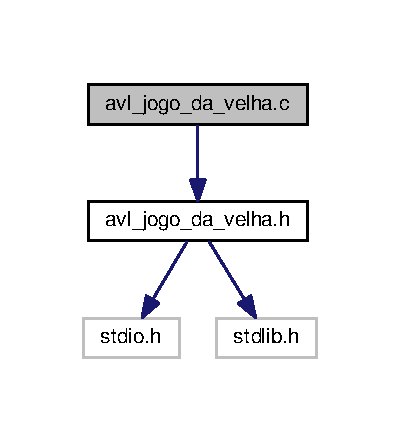
\includegraphics[width=192pt]{avl__jogo__da__velha_8c__incl}
\end{center}
\end{figure}
\subsection*{Functions}
\begin{DoxyCompactItemize}
\item 
void {\bfseries clear} ()\hypertarget{avl__jogo__da__velha_8c_ac8bb3912a3ce86b15842e79d0b421204}{}\label{avl__jogo__da__velha_8c_ac8bb3912a3ce86b15842e79d0b421204}

\item 
int \hyperlink{avl__jogo__da__velha_8c_a95df9e1867414fc6300bba61acbea2dc}{maior} (int esq, int dir)
\begin{DoxyCompactList}\small\item\em Função que ao receber 2 inteiro, retorna o maior deles. \end{DoxyCompactList}\item 
int \hyperlink{avl__jogo__da__velha_8c_ac6bb8a4fc7472c16f5f758a7f7425f68}{altura} (\hyperlink{structnode}{Arvore} $\ast$a)
\begin{DoxyCompactList}\small\item\em Função retorna a altura de uma árvore. \end{DoxyCompactList}\item 
int \hyperlink{avl__jogo__da__velha_8c_a7ee46e52a150b1b20c07acb89bf91eff}{atualizar\+\_\+altura} (\hyperlink{structnode}{Arvore} $\ast$a)
\begin{DoxyCompactList}\small\item\em Função recursiva que atualiza as altura da árvore. \end{DoxyCompactList}\item 
int \hyperlink{avl__jogo__da__velha_8c_aa7d437fe01057d6ba284149c0da2eb05}{balanceamento} (\hyperlink{structnode}{Arvore} $\ast$a)
\begin{DoxyCompactList}\small\item\em Função que retorna a diferença das alturas do nós. \end{DoxyCompactList}\item 
\hyperlink{structnode}{Arvore} $\ast$ \hyperlink{avl__jogo__da__velha_8c_a1d887c6e78f20a742c701e4eef535d0c}{rotacao\+\_\+simples\+\_\+esq} (\hyperlink{structnode}{Arvore} $\ast$r)
\begin{DoxyCompactList}\small\item\em Função que realiza uma rotação simples a esquerda na A\+VL. \end{DoxyCompactList}\item 
\hyperlink{structnode}{Arvore} $\ast$ \hyperlink{avl__jogo__da__velha_8c_aaab988d411edd9c2da9f573470637034}{rotacao\+\_\+simples\+\_\+dir} (\hyperlink{structnode}{Arvore} $\ast$r)
\begin{DoxyCompactList}\small\item\em Função que realiza uma rotação simples a direita na A\+VL. \end{DoxyCompactList}\item 
\hyperlink{structnode}{Arvore} $\ast$ \hyperlink{avl__jogo__da__velha_8c_a6dcd1bb64a374558ddc04d94e4a3c471}{rotacao\+\_\+dupla\+\_\+esq} (\hyperlink{structnode}{Arvore} $\ast$r)
\begin{DoxyCompactList}\small\item\em Função que realiza uma rotação dupla a esquerda na A\+VL. \end{DoxyCompactList}\item 
\hyperlink{structnode}{Arvore} $\ast$ \hyperlink{avl__jogo__da__velha_8c_acc72864ec05d32d4e2976ba36a5b996d}{rotacao\+\_\+dupla\+\_\+dir} (\hyperlink{structnode}{Arvore} $\ast$r)
\begin{DoxyCompactList}\small\item\em Função que realiza uma rotação dupla a direita na A\+VL. \end{DoxyCompactList}\item 
\hyperlink{structnode}{Arvore} $\ast$ \hyperlink{avl__jogo__da__velha_8c_a8ce524b15457a53f5aa1bf0df38c1184}{atualizar\+\_\+fb\+\_\+dir} (\hyperlink{structnode}{Arvore} $\ast$r)
\item 
\hyperlink{structnode}{Arvore} $\ast$ \hyperlink{avl__jogo__da__velha_8c_aa3d5e67559c9a249b23e7f8927842eb7}{atualizar\+\_\+fb\+\_\+esq} (\hyperlink{structnode}{Arvore} $\ast$r)
\item 
\hyperlink{structnode}{Arvore} $\ast$ \hyperlink{avl__jogo__da__velha_8c_a87b15069b0289dade853f446e136d608}{inserir} (\hyperlink{structnode}{Arvore} $\ast$a, int chave, int jogador)
\begin{DoxyCompactList}\small\item\em Insere um novo nó na ávore A\+VL. \end{DoxyCompactList}\item 
\hyperlink{structnode}{Arvore} $\ast$ \hyperlink{avl__jogo__da__velha_8c_a9cd92c535c650a1b614c5d58fb94bfd7}{remover} (\hyperlink{structnode}{Arvore} $\ast$a, int chave)
\begin{DoxyCompactList}\small\item\em Remove um nó da árvore A\+VL baseado na sua chave. \end{DoxyCompactList}\item 
int \hyperlink{avl__jogo__da__velha_8c_a7554598a42d11e8a4fef8f92c36fe13b}{buscar} (\hyperlink{structnode}{Arvore} $\ast$a, int chave)
\begin{DoxyCompactList}\small\item\em Função que encontra um nó específico baseado em sua chave e retorna o valor da variável jogador. \end{DoxyCompactList}\item 
void {\bfseries imprimir\+\_\+in\+\_\+order} (\hyperlink{structnode}{Arvore} $\ast$a, int nivel)\hypertarget{avl__jogo__da__velha_8c_aea57306782b2e4e71a6d3302c221d59f}{}\label{avl__jogo__da__velha_8c_aea57306782b2e4e71a6d3302c221d59f}

\item 
void {\bfseries arvore\+\_\+para\+\_\+vetor} (\hyperlink{structnode}{Arvore} $\ast$a, int $\ast$tabuleiro)\hypertarget{avl__jogo__da__velha_8c_a2f2c94d4950fc1e1f1e596b0801e1a68}{}\label{avl__jogo__da__velha_8c_a2f2c94d4950fc1e1f1e596b0801e1a68}

\item 
void {\bfseries imprimir\+\_\+tabuleiro} (\hyperlink{structnode}{Arvore} $\ast$a)\hypertarget{avl__jogo__da__velha_8c_a24fd6b104ad2346d6eb7fcab9c68f934}{}\label{avl__jogo__da__velha_8c_a24fd6b104ad2346d6eb7fcab9c68f934}

\item 
int \hyperlink{avl__jogo__da__velha_8c_a03c14608eb7cb557075be88d2a193e49}{verifica\+\_\+ganhador} (\hyperlink{structnode}{Arvore} $\ast$a, int jogador)
\begin{DoxyCompactList}\small\item\em Essa função verifica se alguém ganhou o jogo e retorna um inteiro. \end{DoxyCompactList}\item 
int {\bfseries conta\+\_\+nos} (\hyperlink{structnode}{Arvore} $\ast$a)\hypertarget{avl__jogo__da__velha_8c_ad0e19b40f3c84582310a9e7b64d04ed8}{}\label{avl__jogo__da__velha_8c_ad0e19b40f3c84582310a9e7b64d04ed8}

\item 
void {\bfseries calcula\+\_\+passos} (\hyperlink{structnode}{Arvore} $\ast$$\ast$verificacao, \hyperlink{structnode}{Arvore} $\ast$a, \hyperlink{structnode}{Arvore} $\ast$b, int $\ast$passos, int index)\hypertarget{avl__jogo__da__velha_8c_ad6e0af1d45e4f96223f6423c9221faea}{}\label{avl__jogo__da__velha_8c_ad6e0af1d45e4f96223f6423c9221faea}

\item 
\hyperlink{structnode}{Arvore} $\ast$ {\bfseries jogada\+\_\+computador} (\hyperlink{structnode}{Arvore} $\ast$a, \hyperlink{structnode}{Arvore} $\ast$verificacao)\hypertarget{avl__jogo__da__velha_8c_aa30ea74ebd0880f8e2ca5f9857689b9e}{}\label{avl__jogo__da__velha_8c_aa30ea74ebd0880f8e2ca5f9857689b9e}

\item 
int {\bfseries jogada\+\_\+jogador} ()\hypertarget{avl__jogo__da__velha_8c_a5a10ae88f16cca53770a042c5349697f}{}\label{avl__jogo__da__velha_8c_a5a10ae88f16cca53770a042c5349697f}

\item 
int {\bfseries menu\+\_\+principal} ()\hypertarget{avl__jogo__da__velha_8c_a82bec0e1cbde8c596c089e22096c2092}{}\label{avl__jogo__da__velha_8c_a82bec0e1cbde8c596c089e22096c2092}

\end{DoxyCompactItemize}


\subsection{Detailed Description}
Implementação das funções descritas na biblioteca \hyperlink{avl__jogo__da__velha_8h}{avl\+\_\+jogo\+\_\+da\+\_\+velha.\+h}. 

\begin{DoxyAuthor}{Author}
Lucas Ribeiro 
\end{DoxyAuthor}
\begin{DoxyDate}{Date}
25/05/2017 
\end{DoxyDate}


\subsection{Function Documentation}
\index{avl\+\_\+jogo\+\_\+da\+\_\+velha.\+c@{avl\+\_\+jogo\+\_\+da\+\_\+velha.\+c}!altura@{altura}}
\index{altura@{altura}!avl\+\_\+jogo\+\_\+da\+\_\+velha.\+c@{avl\+\_\+jogo\+\_\+da\+\_\+velha.\+c}}
\subsubsection[{\texorpdfstring{altura(\+Arvore $\ast$a)}{altura(Arvore *a)}}]{\setlength{\rightskip}{0pt plus 5cm}int altura (
\begin{DoxyParamCaption}
\item[{{\bf Arvore} $\ast$}]{a}
\end{DoxyParamCaption}
)}\hypertarget{avl__jogo__da__velha_8c_ac6bb8a4fc7472c16f5f758a7f7425f68}{}\label{avl__jogo__da__velha_8c_ac6bb8a4fc7472c16f5f758a7f7425f68}


Função retorna a altura de uma árvore. 

\begin{DoxyPrecond}{Precondition}
O ponteiro para a árvore não deve ter valor N\+U\+LL 
\end{DoxyPrecond}
\begin{DoxyWarning}{Warning}
Caso o pré requisito não seja atendito a funão retornará N\+U\+LL 
\end{DoxyWarning}

\begin{DoxyParams}{Parameters}
{\em a} & Ponteiro que aponta para a árvore A\+VL. \\
\hline
\end{DoxyParams}
\begin{DoxyReturn}{Returns}
Retorna um inteiro que representa 
\end{DoxyReturn}


Here is the caller graph for this function\+:
\nopagebreak
\begin{figure}[H]
\begin{center}
\leavevmode
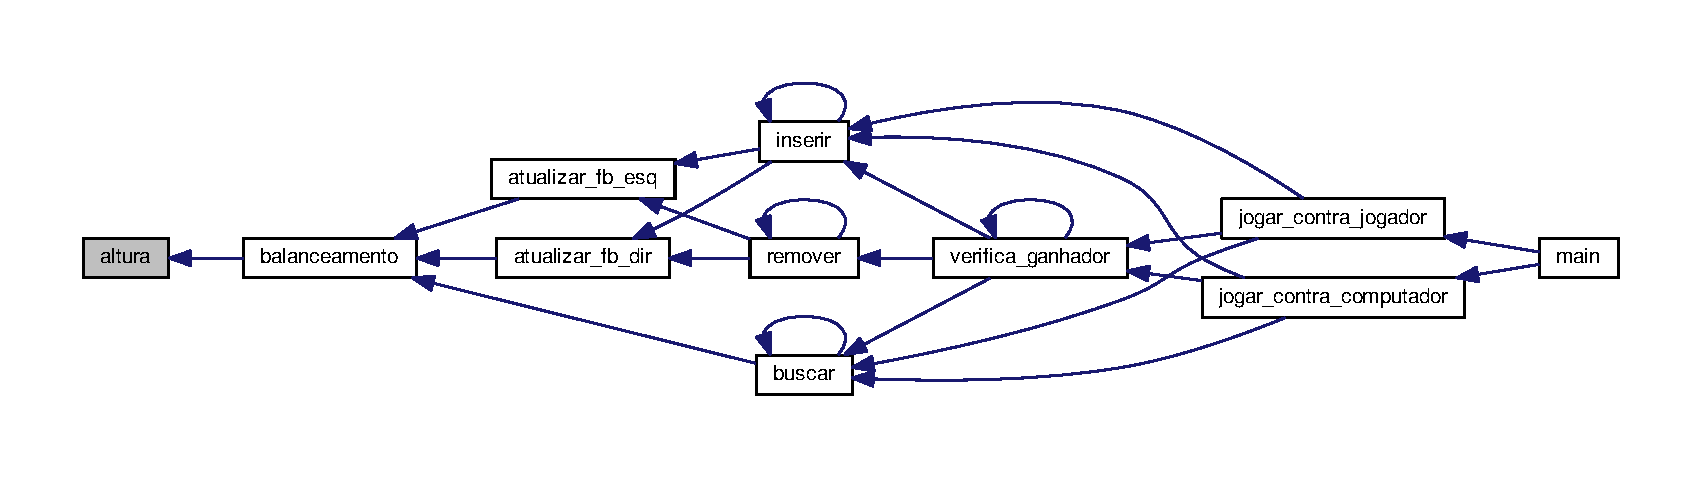
\includegraphics[width=350pt]{avl__jogo__da__velha_8c_ac6bb8a4fc7472c16f5f758a7f7425f68_icgraph}
\end{center}
\end{figure}


\index{avl\+\_\+jogo\+\_\+da\+\_\+velha.\+c@{avl\+\_\+jogo\+\_\+da\+\_\+velha.\+c}!atualizar\+\_\+altura@{atualizar\+\_\+altura}}
\index{atualizar\+\_\+altura@{atualizar\+\_\+altura}!avl\+\_\+jogo\+\_\+da\+\_\+velha.\+c@{avl\+\_\+jogo\+\_\+da\+\_\+velha.\+c}}
\subsubsection[{\texorpdfstring{atualizar\+\_\+altura(\+Arvore $\ast$a)}{atualizar_altura(Arvore *a)}}]{\setlength{\rightskip}{0pt plus 5cm}int atualizar\+\_\+altura (
\begin{DoxyParamCaption}
\item[{{\bf Arvore} $\ast$}]{a}
\end{DoxyParamCaption}
)}\hypertarget{avl__jogo__da__velha_8c_a7ee46e52a150b1b20c07acb89bf91eff}{}\label{avl__jogo__da__velha_8c_a7ee46e52a150b1b20c07acb89bf91eff}


Função recursiva que atualiza as altura da árvore. 


\begin{DoxyParams}{Parameters}
{\em a} & Ponteiro que aponta para o início da A\+VL \\
\hline
\end{DoxyParams}
\begin{DoxyReturn}{Returns}
O retorno inteiro serve para o funcionamento da recursividade. 
\end{DoxyReturn}


Here is the call graph for this function\+:\nopagebreak
\begin{figure}[H]
\begin{center}
\leavevmode
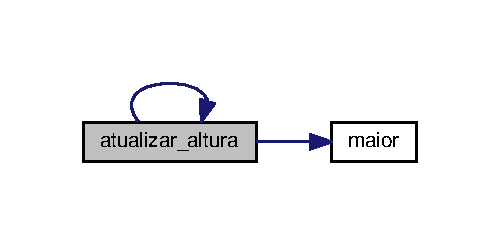
\includegraphics[width=240pt]{avl__jogo__da__velha_8c_a7ee46e52a150b1b20c07acb89bf91eff_cgraph}
\end{center}
\end{figure}




Here is the caller graph for this function\+:
\nopagebreak
\begin{figure}[H]
\begin{center}
\leavevmode
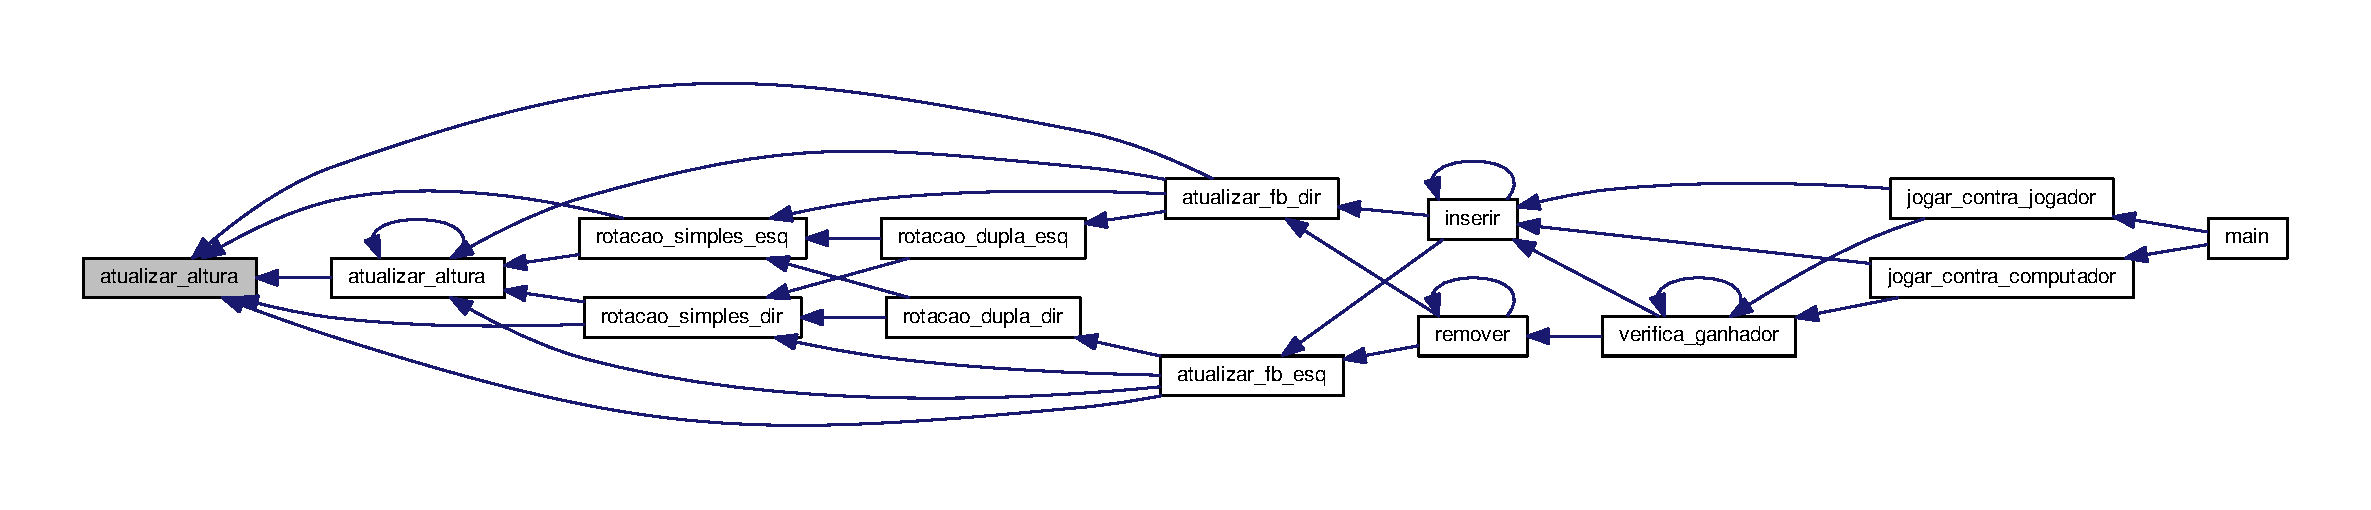
\includegraphics[width=350pt]{avl__jogo__da__velha_8c_a7ee46e52a150b1b20c07acb89bf91eff_icgraph}
\end{center}
\end{figure}


\index{avl\+\_\+jogo\+\_\+da\+\_\+velha.\+c@{avl\+\_\+jogo\+\_\+da\+\_\+velha.\+c}!atualizar\+\_\+fb\+\_\+dir@{atualizar\+\_\+fb\+\_\+dir}}
\index{atualizar\+\_\+fb\+\_\+dir@{atualizar\+\_\+fb\+\_\+dir}!avl\+\_\+jogo\+\_\+da\+\_\+velha.\+c@{avl\+\_\+jogo\+\_\+da\+\_\+velha.\+c}}
\subsubsection[{\texorpdfstring{atualizar\+\_\+fb\+\_\+dir(\+Arvore $\ast$r)}{atualizar_fb_dir(Arvore *r)}}]{\setlength{\rightskip}{0pt plus 5cm}{\bf Arvore} $\ast$ atualizar\+\_\+fb\+\_\+dir (
\begin{DoxyParamCaption}
\item[{{\bf Arvore} $\ast$}]{r}
\end{DoxyParamCaption}
)}\hypertarget{avl__jogo__da__velha_8c_a8ce524b15457a53f5aa1bf0df38c1184}{}\label{avl__jogo__da__velha_8c_a8ce524b15457a53f5aa1bf0df38c1184}
Função que atualiza a altura e faz o balanceamento dos nós casos os dá direita estejam desbalanceados. 
\begin{DoxyParams}{Parameters}
{\em r} & Ponteiro que aponta para um nó da árvore A\+VL. \\
\hline
\end{DoxyParams}
\begin{DoxyReturn}{Returns}
Retorna o ponteiro para o nó após as devidas atualizações. 
\end{DoxyReturn}


Here is the call graph for this function\+:\nopagebreak
\begin{figure}[H]
\begin{center}
\leavevmode
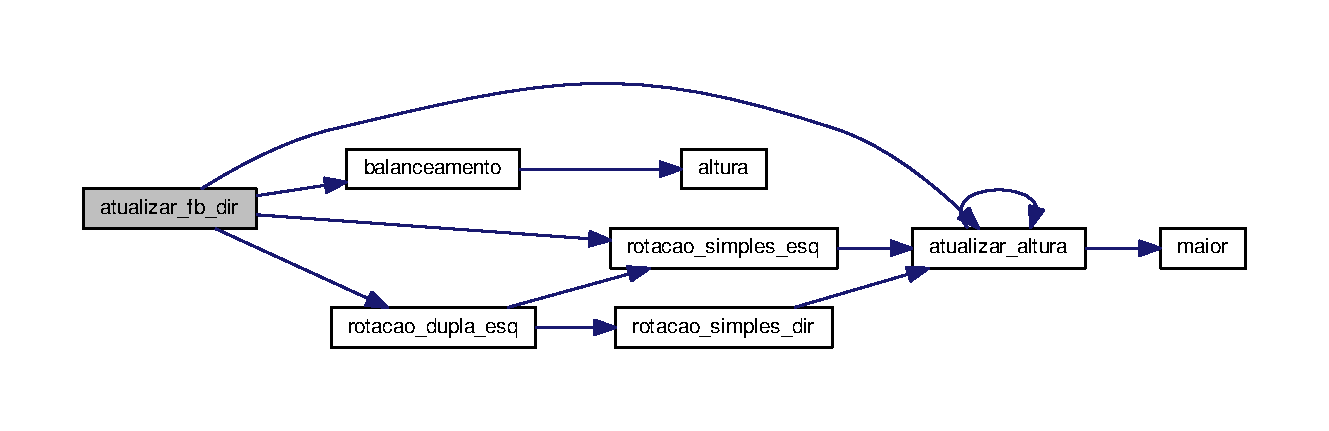
\includegraphics[width=350pt]{avl__jogo__da__velha_8c_a8ce524b15457a53f5aa1bf0df38c1184_cgraph}
\end{center}
\end{figure}




Here is the caller graph for this function\+:
\nopagebreak
\begin{figure}[H]
\begin{center}
\leavevmode
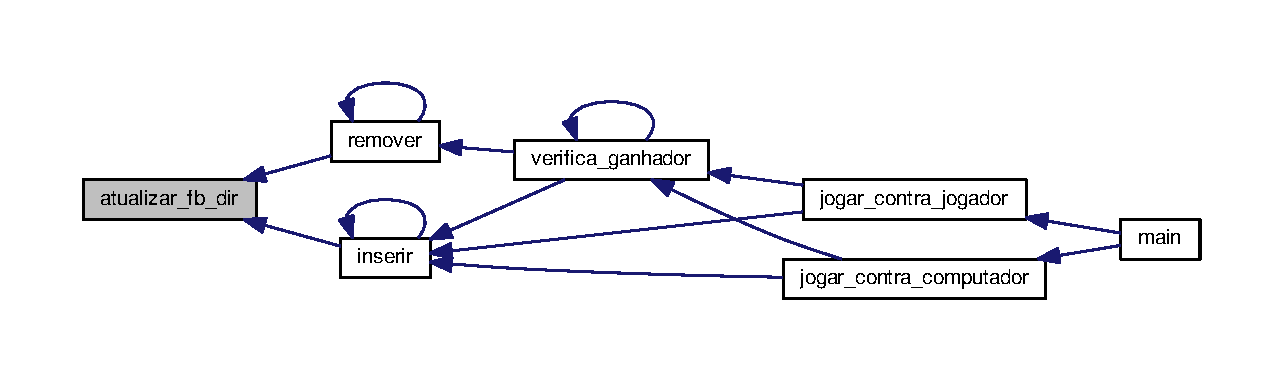
\includegraphics[width=350pt]{avl__jogo__da__velha_8c_a8ce524b15457a53f5aa1bf0df38c1184_icgraph}
\end{center}
\end{figure}


\index{avl\+\_\+jogo\+\_\+da\+\_\+velha.\+c@{avl\+\_\+jogo\+\_\+da\+\_\+velha.\+c}!atualizar\+\_\+fb\+\_\+esq@{atualizar\+\_\+fb\+\_\+esq}}
\index{atualizar\+\_\+fb\+\_\+esq@{atualizar\+\_\+fb\+\_\+esq}!avl\+\_\+jogo\+\_\+da\+\_\+velha.\+c@{avl\+\_\+jogo\+\_\+da\+\_\+velha.\+c}}
\subsubsection[{\texorpdfstring{atualizar\+\_\+fb\+\_\+esq(\+Arvore $\ast$r)}{atualizar_fb_esq(Arvore *r)}}]{\setlength{\rightskip}{0pt plus 5cm}{\bf Arvore} $\ast$ atualizar\+\_\+fb\+\_\+esq (
\begin{DoxyParamCaption}
\item[{{\bf Arvore} $\ast$}]{r}
\end{DoxyParamCaption}
)}\hypertarget{avl__jogo__da__velha_8c_aa3d5e67559c9a249b23e7f8927842eb7}{}\label{avl__jogo__da__velha_8c_aa3d5e67559c9a249b23e7f8927842eb7}
Função que atualiza a altura e faz o balancemanto dos nós casos os daá esquerda estejam desbalanceados. 
\begin{DoxyParams}{Parameters}
{\em r} & Ponteiro que aponta para um nó da árvore A\+VL. \\
\hline
\end{DoxyParams}
\begin{DoxyReturn}{Returns}
Retorna o ponteiro para o nó após as devidas alterações feitas. 
\end{DoxyReturn}


Here is the call graph for this function\+:\nopagebreak
\begin{figure}[H]
\begin{center}
\leavevmode
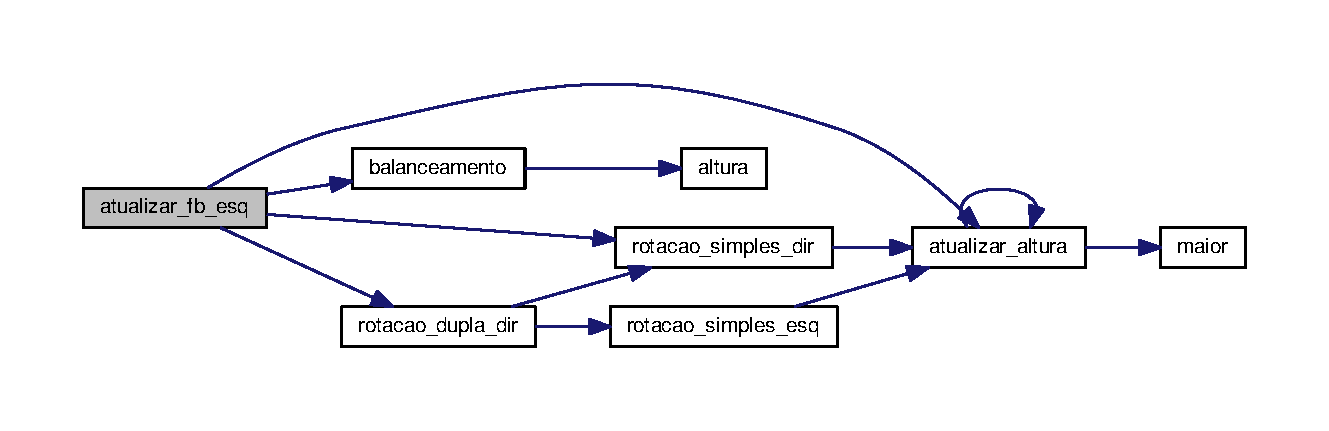
\includegraphics[width=350pt]{avl__jogo__da__velha_8c_aa3d5e67559c9a249b23e7f8927842eb7_cgraph}
\end{center}
\end{figure}




Here is the caller graph for this function\+:
\nopagebreak
\begin{figure}[H]
\begin{center}
\leavevmode
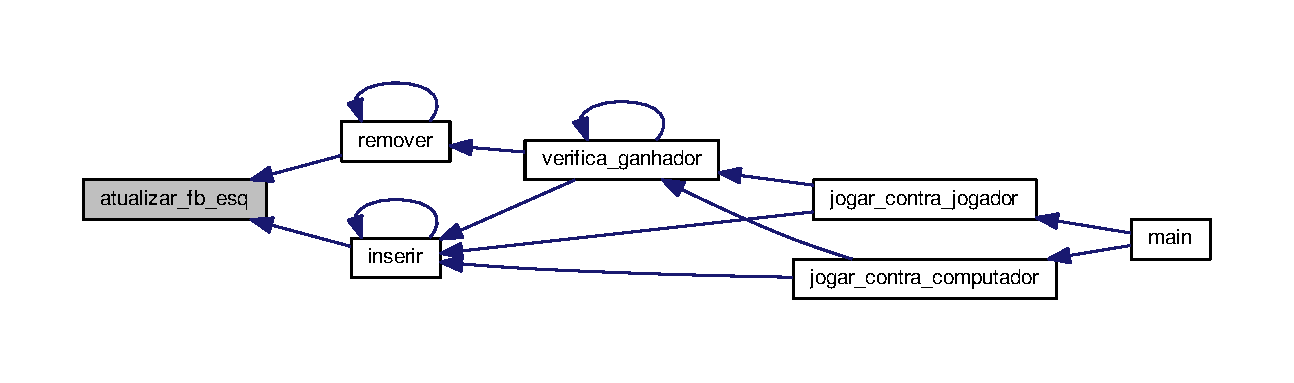
\includegraphics[width=350pt]{avl__jogo__da__velha_8c_aa3d5e67559c9a249b23e7f8927842eb7_icgraph}
\end{center}
\end{figure}


\index{avl\+\_\+jogo\+\_\+da\+\_\+velha.\+c@{avl\+\_\+jogo\+\_\+da\+\_\+velha.\+c}!balanceamento@{balanceamento}}
\index{balanceamento@{balanceamento}!avl\+\_\+jogo\+\_\+da\+\_\+velha.\+c@{avl\+\_\+jogo\+\_\+da\+\_\+velha.\+c}}
\subsubsection[{\texorpdfstring{balanceamento(\+Arvore $\ast$a)}{balanceamento(Arvore *a)}}]{\setlength{\rightskip}{0pt plus 5cm}int balanceamento (
\begin{DoxyParamCaption}
\item[{{\bf Arvore} $\ast$}]{a}
\end{DoxyParamCaption}
)}\hypertarget{avl__jogo__da__velha_8c_aa7d437fe01057d6ba284149c0da2eb05}{}\label{avl__jogo__da__velha_8c_aa7d437fe01057d6ba284149c0da2eb05}


Função que retorna a diferença das alturas do nós. 

A função de balancemanto serve para retornar um valor que indica se o nó está balanceado ou não, retornando um valor que vária de -\/2 a 2. 
\begin{DoxyParams}{Parameters}
{\em a} & Ponteiro que aponta para um nó da árvore A\+VL; \\
\hline
\end{DoxyParams}
\begin{DoxyReturn}{Returns}
Retorna o valor do balanceamento 
\end{DoxyReturn}


Here is the call graph for this function\+:\nopagebreak
\begin{figure}[H]
\begin{center}
\leavevmode
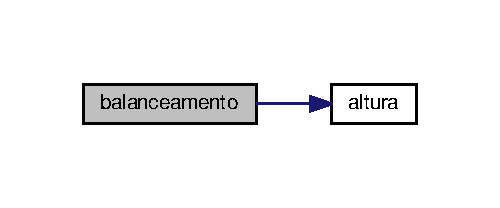
\includegraphics[width=240pt]{avl__jogo__da__velha_8c_aa7d437fe01057d6ba284149c0da2eb05_cgraph}
\end{center}
\end{figure}




Here is the caller graph for this function\+:
\nopagebreak
\begin{figure}[H]
\begin{center}
\leavevmode
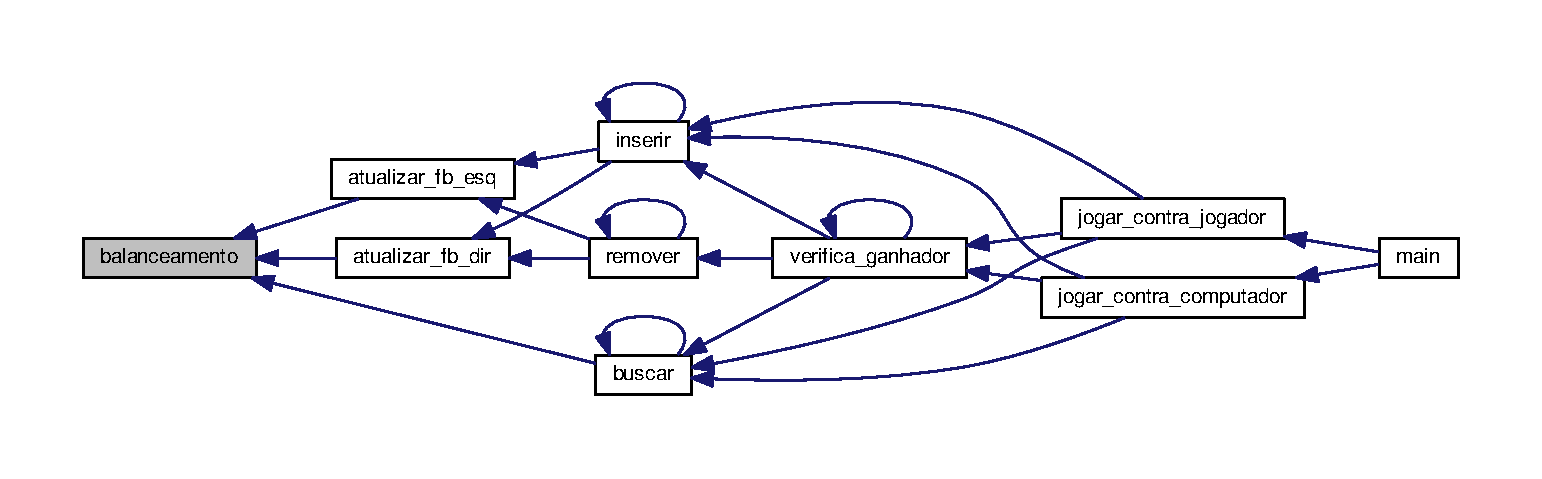
\includegraphics[width=350pt]{avl__jogo__da__velha_8c_aa7d437fe01057d6ba284149c0da2eb05_icgraph}
\end{center}
\end{figure}


\index{avl\+\_\+jogo\+\_\+da\+\_\+velha.\+c@{avl\+\_\+jogo\+\_\+da\+\_\+velha.\+c}!buscar@{buscar}}
\index{buscar@{buscar}!avl\+\_\+jogo\+\_\+da\+\_\+velha.\+c@{avl\+\_\+jogo\+\_\+da\+\_\+velha.\+c}}
\subsubsection[{\texorpdfstring{buscar(\+Arvore $\ast$a, int chave)}{buscar(Arvore *a, int chave)}}]{\setlength{\rightskip}{0pt plus 5cm}int buscar (
\begin{DoxyParamCaption}
\item[{{\bf Arvore} $\ast$}]{a, }
\item[{int}]{chave}
\end{DoxyParamCaption}
)}\hypertarget{avl__jogo__da__velha_8c_a7554598a42d11e8a4fef8f92c36fe13b}{}\label{avl__jogo__da__velha_8c_a7554598a42d11e8a4fef8f92c36fe13b}


Função que encontra um nó específico baseado em sua chave e retorna o valor da variável jogador. 


\begin{DoxyParams}{Parameters}
{\em a} & Ponteiro que aponta para a ávore em que se deseja buscar. \\
\hline
{\em chave} & Inteiro que representa a chave do nó que se deseja achar. \\
\hline
\end{DoxyParams}
\begin{DoxyReturn}{Returns}
Retorna um inteiro com o mesmo valor da variável jogador do nó que se buscava. 
\end{DoxyReturn}


Here is the call graph for this function\+:\nopagebreak
\begin{figure}[H]
\begin{center}
\leavevmode
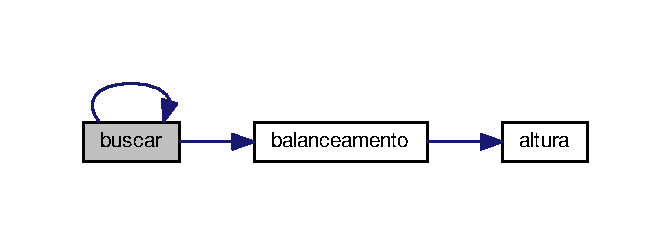
\includegraphics[width=322pt]{avl__jogo__da__velha_8c_a7554598a42d11e8a4fef8f92c36fe13b_cgraph}
\end{center}
\end{figure}




Here is the caller graph for this function\+:
\nopagebreak
\begin{figure}[H]
\begin{center}
\leavevmode
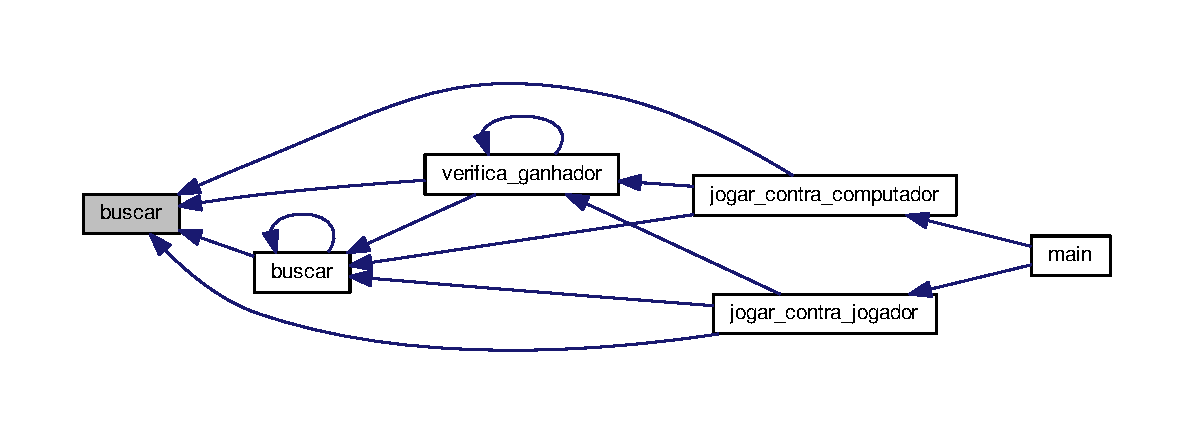
\includegraphics[width=350pt]{avl__jogo__da__velha_8c_a7554598a42d11e8a4fef8f92c36fe13b_icgraph}
\end{center}
\end{figure}


\index{avl\+\_\+jogo\+\_\+da\+\_\+velha.\+c@{avl\+\_\+jogo\+\_\+da\+\_\+velha.\+c}!inserir@{inserir}}
\index{inserir@{inserir}!avl\+\_\+jogo\+\_\+da\+\_\+velha.\+c@{avl\+\_\+jogo\+\_\+da\+\_\+velha.\+c}}
\subsubsection[{\texorpdfstring{inserir(\+Arvore $\ast$a, int chave, int jogador)}{inserir(Arvore *a, int chave, int jogador)}}]{\setlength{\rightskip}{0pt plus 5cm}{\bf Arvore} $\ast$ inserir (
\begin{DoxyParamCaption}
\item[{{\bf Arvore} $\ast$}]{a, }
\item[{int}]{chave, }
\item[{int}]{jogador}
\end{DoxyParamCaption}
)}\hypertarget{avl__jogo__da__velha_8c_a87b15069b0289dade853f446e136d608}{}\label{avl__jogo__da__velha_8c_a87b15069b0289dade853f446e136d608}


Insere um novo nó na ávore A\+VL. 


\begin{DoxyParams}{Parameters}
{\em a} & É um ponteiro que representa a árvore onde se quer inserir. \\
\hline
{\em chave} & É um inteiro que representa o valor do nó. \\
\hline
{\em jogador} & É um inteiro que representa o jogador que fez a jogada. \\
\hline
\end{DoxyParams}
\begin{DoxyReturn}{Returns}
Retorna o ponteiro para árvore após a inserção ter sido feita. 
\end{DoxyReturn}


Here is the call graph for this function\+:\nopagebreak
\begin{figure}[H]
\begin{center}
\leavevmode
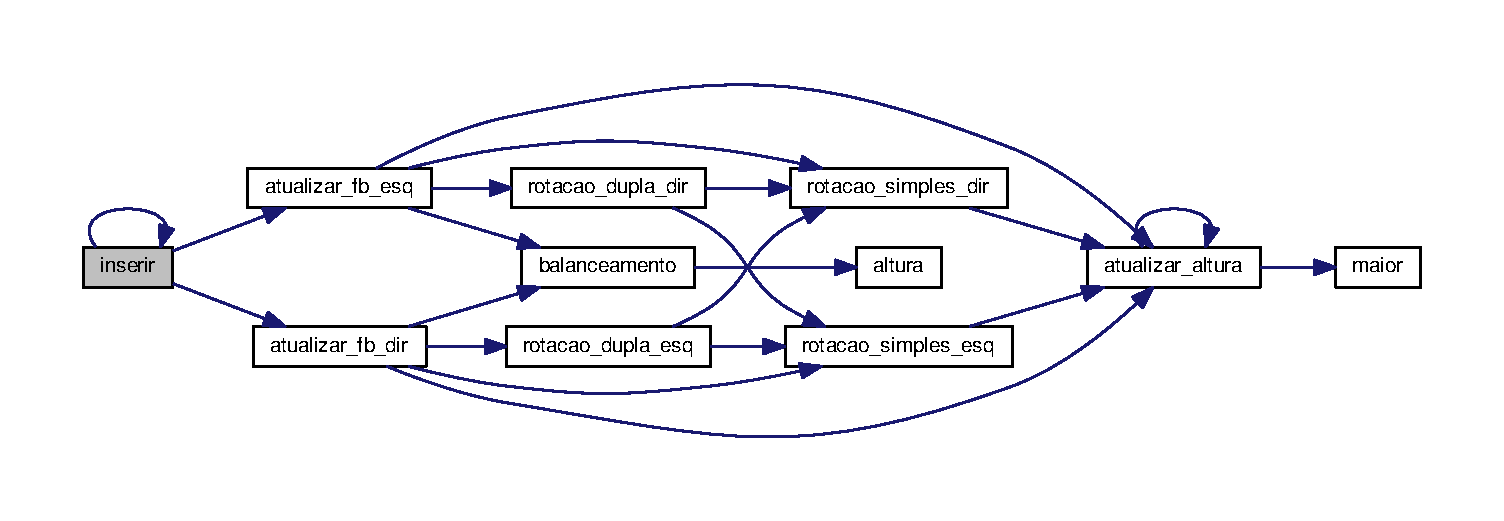
\includegraphics[width=350pt]{avl__jogo__da__velha_8c_a87b15069b0289dade853f446e136d608_cgraph}
\end{center}
\end{figure}




Here is the caller graph for this function\+:
\nopagebreak
\begin{figure}[H]
\begin{center}
\leavevmode
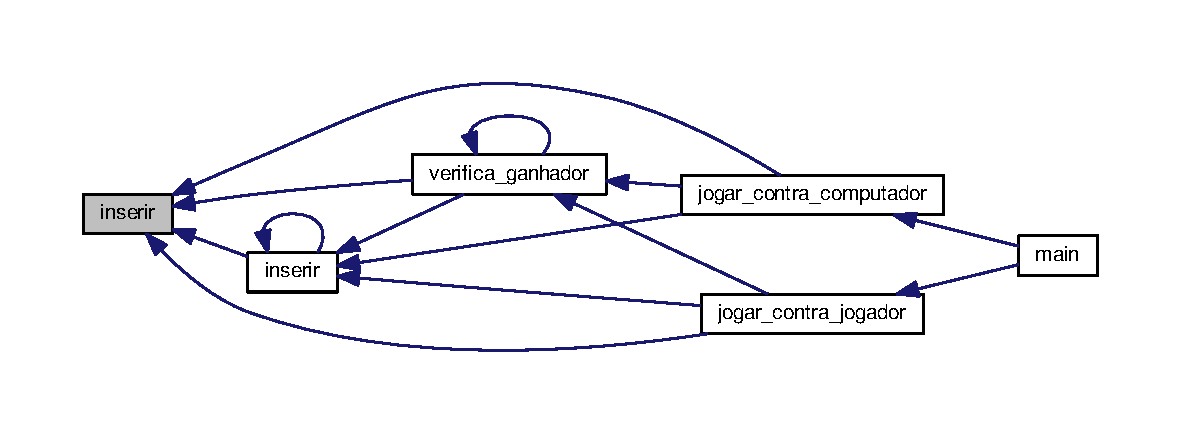
\includegraphics[width=350pt]{avl__jogo__da__velha_8c_a87b15069b0289dade853f446e136d608_icgraph}
\end{center}
\end{figure}


\index{avl\+\_\+jogo\+\_\+da\+\_\+velha.\+c@{avl\+\_\+jogo\+\_\+da\+\_\+velha.\+c}!maior@{maior}}
\index{maior@{maior}!avl\+\_\+jogo\+\_\+da\+\_\+velha.\+c@{avl\+\_\+jogo\+\_\+da\+\_\+velha.\+c}}
\subsubsection[{\texorpdfstring{maior(int esq, int dir)}{maior(int esq, int dir)}}]{\setlength{\rightskip}{0pt plus 5cm}int maior (
\begin{DoxyParamCaption}
\item[{int}]{esq, }
\item[{int}]{dir}
\end{DoxyParamCaption}
)}\hypertarget{avl__jogo__da__velha_8c_a95df9e1867414fc6300bba61acbea2dc}{}\label{avl__jogo__da__velha_8c_a95df9e1867414fc6300bba61acbea2dc}


Função que ao receber 2 inteiro, retorna o maior deles. 


\begin{DoxyParams}{Parameters}
{\em esq} & Inteiro que representa o valor a esquerda da A\+VL. \\
\hline
{\em dir} & Inteiro que representa o valor a direita da A\+VL. \\
\hline
\end{DoxyParams}
\begin{DoxyReturn}{Returns}
Retorno inteiro que representa o maior de ambos os valores. 
\end{DoxyReturn}


Here is the caller graph for this function\+:
\nopagebreak
\begin{figure}[H]
\begin{center}
\leavevmode
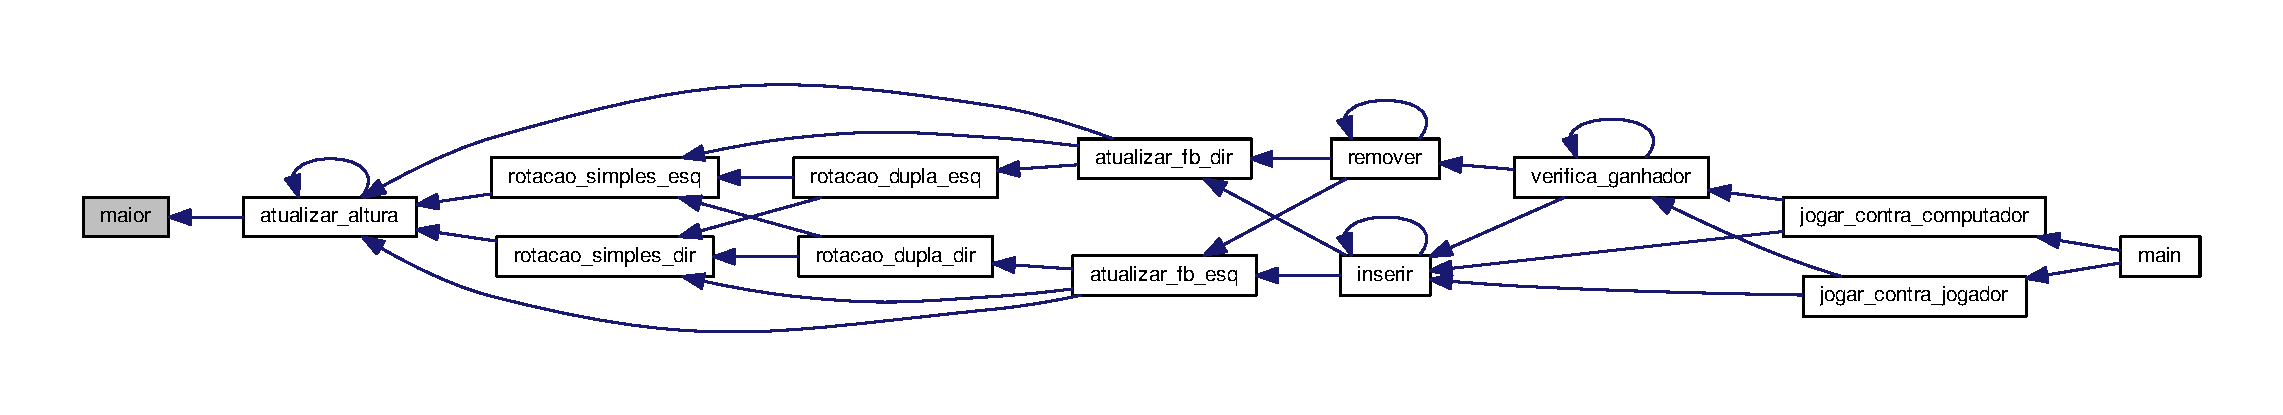
\includegraphics[width=350pt]{avl__jogo__da__velha_8c_a95df9e1867414fc6300bba61acbea2dc_icgraph}
\end{center}
\end{figure}


\index{avl\+\_\+jogo\+\_\+da\+\_\+velha.\+c@{avl\+\_\+jogo\+\_\+da\+\_\+velha.\+c}!remover@{remover}}
\index{remover@{remover}!avl\+\_\+jogo\+\_\+da\+\_\+velha.\+c@{avl\+\_\+jogo\+\_\+da\+\_\+velha.\+c}}
\subsubsection[{\texorpdfstring{remover(\+Arvore $\ast$a, int chave)}{remover(Arvore *a, int chave)}}]{\setlength{\rightskip}{0pt plus 5cm}{\bf Arvore} $\ast$ remover (
\begin{DoxyParamCaption}
\item[{{\bf Arvore} $\ast$}]{a, }
\item[{int}]{chave}
\end{DoxyParamCaption}
)}\hypertarget{avl__jogo__da__velha_8c_a9cd92c535c650a1b614c5d58fb94bfd7}{}\label{avl__jogo__da__velha_8c_a9cd92c535c650a1b614c5d58fb94bfd7}


Remove um nó da árvore A\+VL baseado na sua chave. 


\begin{DoxyParams}{Parameters}
{\em a} & É um ponteiro que aponta para a árvore ao qual se deseja remover o nó. \\
\hline
{\em chave} & É um inteiro que representa a chave do nó que se pretende remover \\
\hline
\end{DoxyParams}
\begin{DoxyReturn}{Returns}
Retorna o ponteiro para a árvore, após ter sido removido o nó. 
\end{DoxyReturn}


Here is the call graph for this function\+:\nopagebreak
\begin{figure}[H]
\begin{center}
\leavevmode
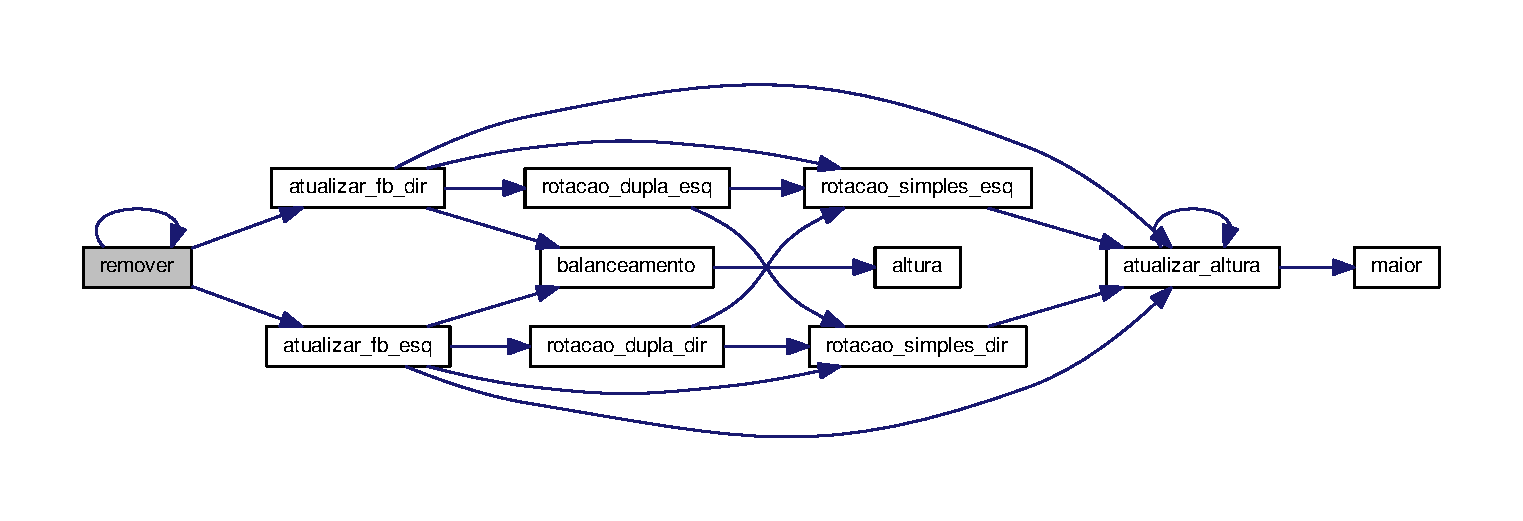
\includegraphics[width=350pt]{avl__jogo__da__velha_8c_a9cd92c535c650a1b614c5d58fb94bfd7_cgraph}
\end{center}
\end{figure}




Here is the caller graph for this function\+:
\nopagebreak
\begin{figure}[H]
\begin{center}
\leavevmode
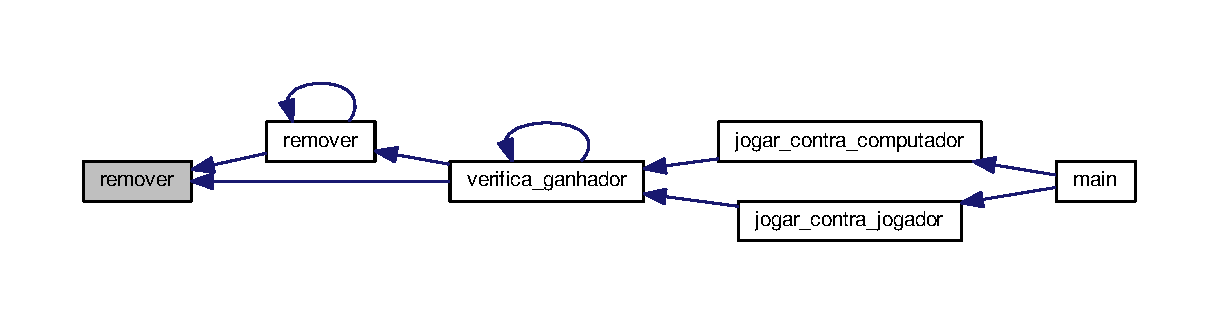
\includegraphics[width=350pt]{avl__jogo__da__velha_8c_a9cd92c535c650a1b614c5d58fb94bfd7_icgraph}
\end{center}
\end{figure}


\index{avl\+\_\+jogo\+\_\+da\+\_\+velha.\+c@{avl\+\_\+jogo\+\_\+da\+\_\+velha.\+c}!rotacao\+\_\+dupla\+\_\+dir@{rotacao\+\_\+dupla\+\_\+dir}}
\index{rotacao\+\_\+dupla\+\_\+dir@{rotacao\+\_\+dupla\+\_\+dir}!avl\+\_\+jogo\+\_\+da\+\_\+velha.\+c@{avl\+\_\+jogo\+\_\+da\+\_\+velha.\+c}}
\subsubsection[{\texorpdfstring{rotacao\+\_\+dupla\+\_\+dir(\+Arvore $\ast$r)}{rotacao_dupla_dir(Arvore *r)}}]{\setlength{\rightskip}{0pt plus 5cm}{\bf Arvore} $\ast$ rotacao\+\_\+dupla\+\_\+dir (
\begin{DoxyParamCaption}
\item[{{\bf Arvore} $\ast$}]{r}
\end{DoxyParamCaption}
)}\hypertarget{avl__jogo__da__velha_8c_acc72864ec05d32d4e2976ba36a5b996d}{}\label{avl__jogo__da__velha_8c_acc72864ec05d32d4e2976ba36a5b996d}


Função que realiza uma rotação dupla a direita na A\+VL. 


\begin{DoxyParams}{Parameters}
{\em r} & Ponteiro que aponta para um nó da árvore A\+VL. \\
\hline
\end{DoxyParams}
\begin{DoxyReturn}{Returns}
Retorna o ponteiro do nó da A\+VL após a rotação feita. 
\end{DoxyReturn}


Here is the call graph for this function\+:\nopagebreak
\begin{figure}[H]
\begin{center}
\leavevmode
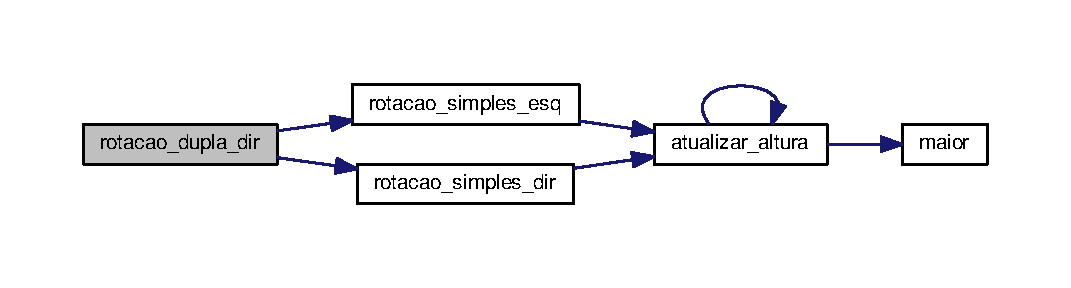
\includegraphics[width=350pt]{avl__jogo__da__velha_8c_acc72864ec05d32d4e2976ba36a5b996d_cgraph}
\end{center}
\end{figure}




Here is the caller graph for this function\+:
\nopagebreak
\begin{figure}[H]
\begin{center}
\leavevmode
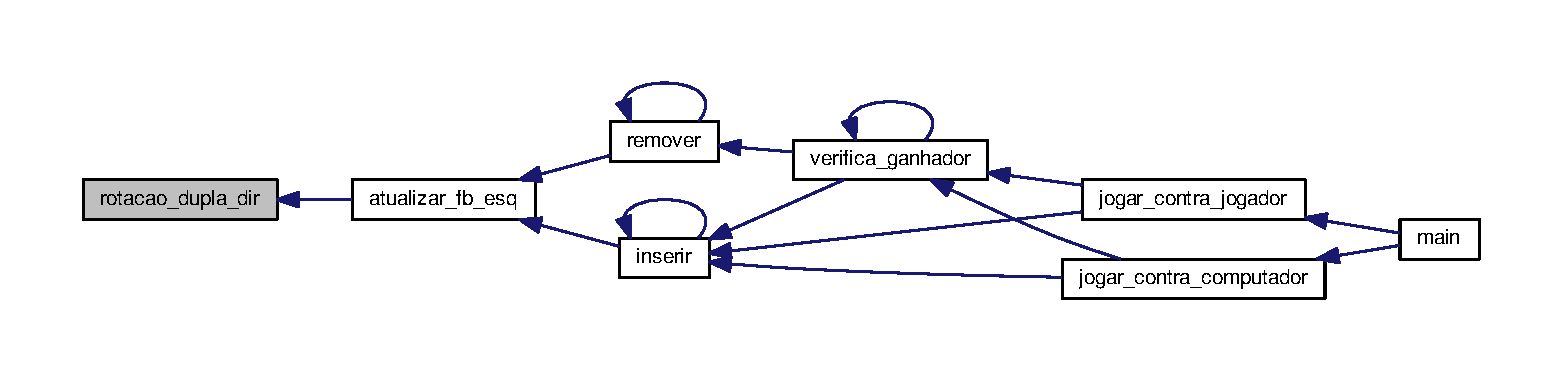
\includegraphics[width=350pt]{avl__jogo__da__velha_8c_acc72864ec05d32d4e2976ba36a5b996d_icgraph}
\end{center}
\end{figure}


\index{avl\+\_\+jogo\+\_\+da\+\_\+velha.\+c@{avl\+\_\+jogo\+\_\+da\+\_\+velha.\+c}!rotacao\+\_\+dupla\+\_\+esq@{rotacao\+\_\+dupla\+\_\+esq}}
\index{rotacao\+\_\+dupla\+\_\+esq@{rotacao\+\_\+dupla\+\_\+esq}!avl\+\_\+jogo\+\_\+da\+\_\+velha.\+c@{avl\+\_\+jogo\+\_\+da\+\_\+velha.\+c}}
\subsubsection[{\texorpdfstring{rotacao\+\_\+dupla\+\_\+esq(\+Arvore $\ast$r)}{rotacao_dupla_esq(Arvore *r)}}]{\setlength{\rightskip}{0pt plus 5cm}{\bf Arvore} $\ast$ rotacao\+\_\+dupla\+\_\+esq (
\begin{DoxyParamCaption}
\item[{{\bf Arvore} $\ast$}]{r}
\end{DoxyParamCaption}
)}\hypertarget{avl__jogo__da__velha_8c_a6dcd1bb64a374558ddc04d94e4a3c471}{}\label{avl__jogo__da__velha_8c_a6dcd1bb64a374558ddc04d94e4a3c471}


Função que realiza uma rotação dupla a esquerda na A\+VL. 


\begin{DoxyParams}{Parameters}
{\em r} & Ponteiro que aponta para um nó da árvore A\+VL. \\
\hline
\end{DoxyParams}
\begin{DoxyReturn}{Returns}
Retorna o ponteiro do nó da A\+VL após a rotação feita. 
\end{DoxyReturn}


Here is the call graph for this function\+:\nopagebreak
\begin{figure}[H]
\begin{center}
\leavevmode
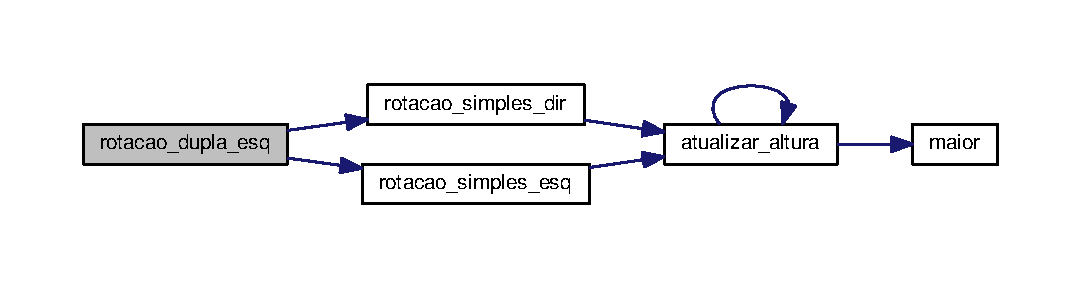
\includegraphics[width=350pt]{avl__jogo__da__velha_8c_a6dcd1bb64a374558ddc04d94e4a3c471_cgraph}
\end{center}
\end{figure}




Here is the caller graph for this function\+:
\nopagebreak
\begin{figure}[H]
\begin{center}
\leavevmode
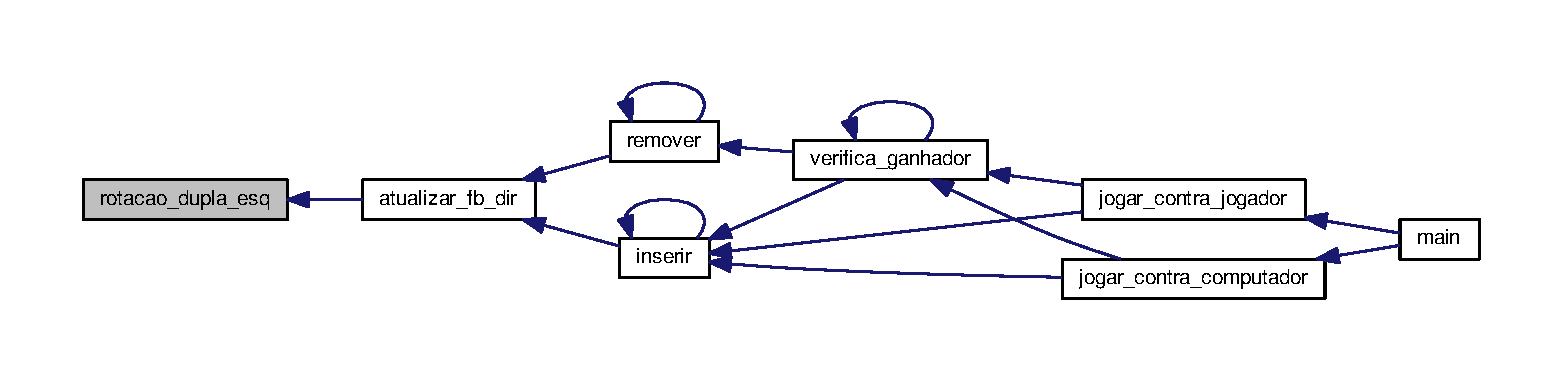
\includegraphics[width=350pt]{avl__jogo__da__velha_8c_a6dcd1bb64a374558ddc04d94e4a3c471_icgraph}
\end{center}
\end{figure}


\index{avl\+\_\+jogo\+\_\+da\+\_\+velha.\+c@{avl\+\_\+jogo\+\_\+da\+\_\+velha.\+c}!rotacao\+\_\+simples\+\_\+dir@{rotacao\+\_\+simples\+\_\+dir}}
\index{rotacao\+\_\+simples\+\_\+dir@{rotacao\+\_\+simples\+\_\+dir}!avl\+\_\+jogo\+\_\+da\+\_\+velha.\+c@{avl\+\_\+jogo\+\_\+da\+\_\+velha.\+c}}
\subsubsection[{\texorpdfstring{rotacao\+\_\+simples\+\_\+dir(\+Arvore $\ast$r)}{rotacao_simples_dir(Arvore *r)}}]{\setlength{\rightskip}{0pt plus 5cm}{\bf Arvore} $\ast$ rotacao\+\_\+simples\+\_\+dir (
\begin{DoxyParamCaption}
\item[{{\bf Arvore} $\ast$}]{r}
\end{DoxyParamCaption}
)}\hypertarget{avl__jogo__da__velha_8c_aaab988d411edd9c2da9f573470637034}{}\label{avl__jogo__da__velha_8c_aaab988d411edd9c2da9f573470637034}


Função que realiza uma rotação simples a direita na A\+VL. 


\begin{DoxyParams}{Parameters}
{\em r} & Ponteiro que aponta para um nó da árvore A\+VL. \\
\hline
\end{DoxyParams}
\begin{DoxyReturn}{Returns}
Retorna o ponteiro do nó da A\+VL após a rotação feita 
\end{DoxyReturn}


Here is the call graph for this function\+:\nopagebreak
\begin{figure}[H]
\begin{center}
\leavevmode
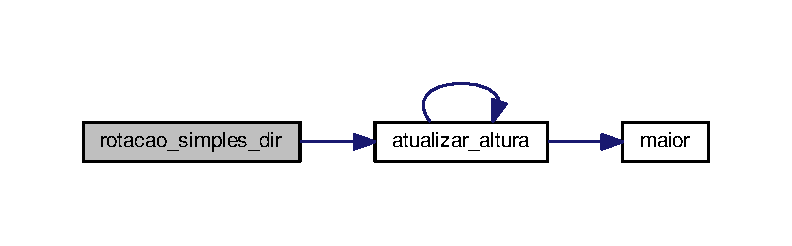
\includegraphics[width=350pt]{avl__jogo__da__velha_8c_aaab988d411edd9c2da9f573470637034_cgraph}
\end{center}
\end{figure}




Here is the caller graph for this function\+:
\nopagebreak
\begin{figure}[H]
\begin{center}
\leavevmode
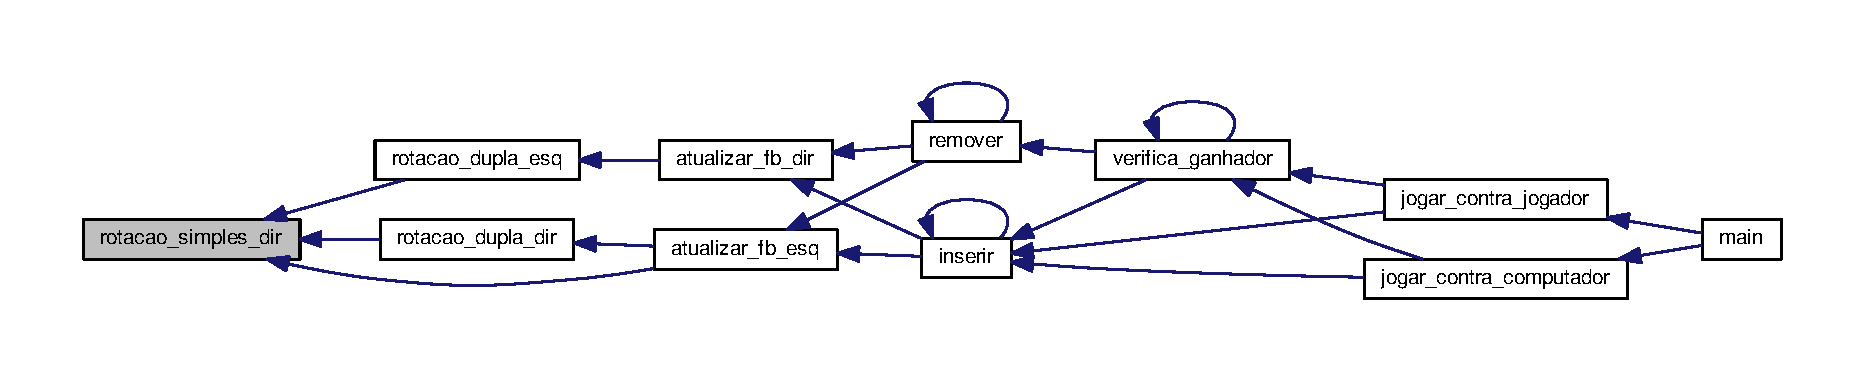
\includegraphics[width=350pt]{avl__jogo__da__velha_8c_aaab988d411edd9c2da9f573470637034_icgraph}
\end{center}
\end{figure}


\index{avl\+\_\+jogo\+\_\+da\+\_\+velha.\+c@{avl\+\_\+jogo\+\_\+da\+\_\+velha.\+c}!rotacao\+\_\+simples\+\_\+esq@{rotacao\+\_\+simples\+\_\+esq}}
\index{rotacao\+\_\+simples\+\_\+esq@{rotacao\+\_\+simples\+\_\+esq}!avl\+\_\+jogo\+\_\+da\+\_\+velha.\+c@{avl\+\_\+jogo\+\_\+da\+\_\+velha.\+c}}
\subsubsection[{\texorpdfstring{rotacao\+\_\+simples\+\_\+esq(\+Arvore $\ast$r)}{rotacao_simples_esq(Arvore *r)}}]{\setlength{\rightskip}{0pt plus 5cm}{\bf Arvore} $\ast$ rotacao\+\_\+simples\+\_\+esq (
\begin{DoxyParamCaption}
\item[{{\bf Arvore} $\ast$}]{r}
\end{DoxyParamCaption}
)}\hypertarget{avl__jogo__da__velha_8c_a1d887c6e78f20a742c701e4eef535d0c}{}\label{avl__jogo__da__velha_8c_a1d887c6e78f20a742c701e4eef535d0c}


Função que realiza uma rotação simples a esquerda na A\+VL. 


\begin{DoxyParams}{Parameters}
{\em r} & Ponteiro que aponta para um nó da árvore A\+V\+L! \\
\hline
\end{DoxyParams}
\begin{DoxyReturn}{Returns}
Retorna o ponteiro do nó da A\+VL após a rotação feita 
\end{DoxyReturn}


Here is the call graph for this function\+:\nopagebreak
\begin{figure}[H]
\begin{center}
\leavevmode
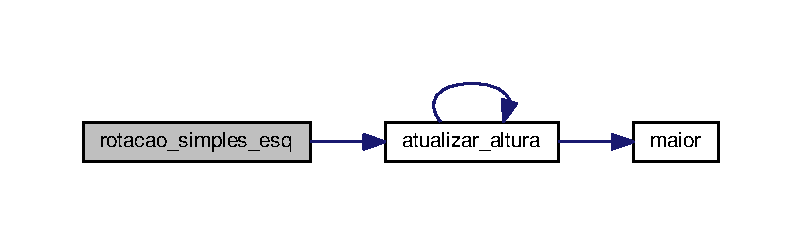
\includegraphics[width=350pt]{avl__jogo__da__velha_8c_a1d887c6e78f20a742c701e4eef535d0c_cgraph}
\end{center}
\end{figure}




Here is the caller graph for this function\+:
\nopagebreak
\begin{figure}[H]
\begin{center}
\leavevmode
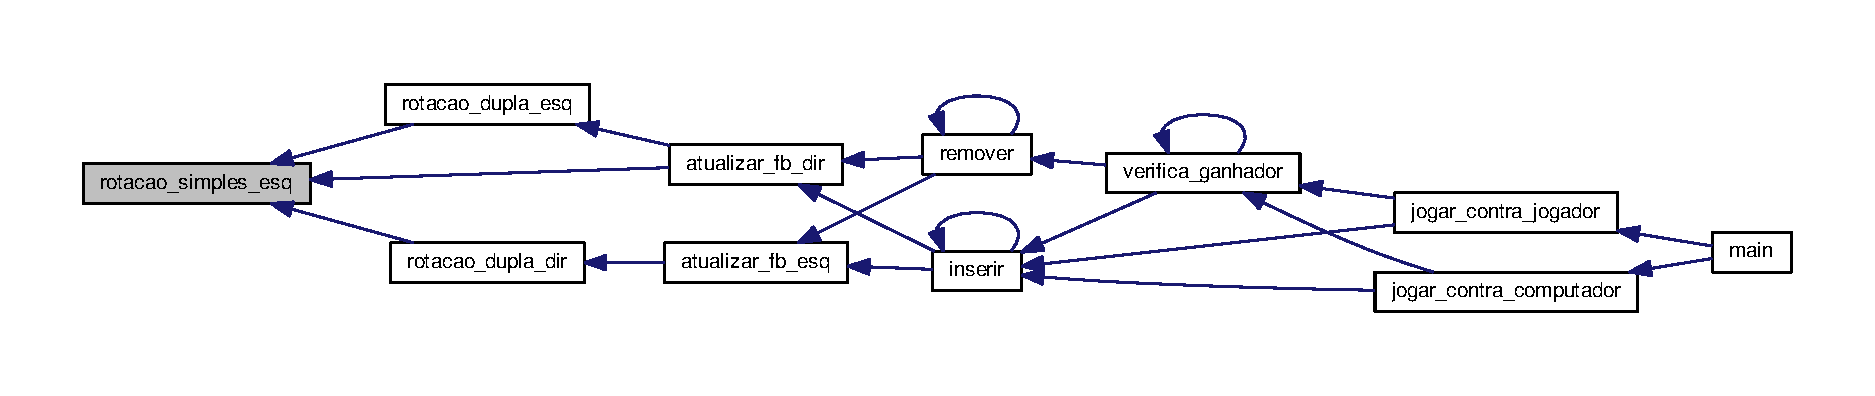
\includegraphics[width=350pt]{avl__jogo__da__velha_8c_a1d887c6e78f20a742c701e4eef535d0c_icgraph}
\end{center}
\end{figure}


\index{avl\+\_\+jogo\+\_\+da\+\_\+velha.\+c@{avl\+\_\+jogo\+\_\+da\+\_\+velha.\+c}!verifica\+\_\+ganhador@{verifica\+\_\+ganhador}}
\index{verifica\+\_\+ganhador@{verifica\+\_\+ganhador}!avl\+\_\+jogo\+\_\+da\+\_\+velha.\+c@{avl\+\_\+jogo\+\_\+da\+\_\+velha.\+c}}
\subsubsection[{\texorpdfstring{verifica\+\_\+ganhador(\+Arvore $\ast$a, int jogador)}{verifica_ganhador(Arvore *a, int jogador)}}]{\setlength{\rightskip}{0pt plus 5cm}int verifica\+\_\+ganhador (
\begin{DoxyParamCaption}
\item[{{\bf Arvore} $\ast$}]{a, }
\item[{int}]{jogador}
\end{DoxyParamCaption}
)}\hypertarget{avl__jogo__da__velha_8c_a03c14608eb7cb557075be88d2a193e49}{}\label{avl__jogo__da__velha_8c_a03c14608eb7cb557075be88d2a193e49}


Essa função verifica se alguém ganhou o jogo e retorna um inteiro. 


\begin{DoxyParams}{Parameters}
{\em a} & É um ponteiro para a árvore A\+VL. \\
\hline
{\em jogador} & É um inteiro que representa qual jogador se está verificando. \\
\hline
\end{DoxyParams}
\begin{DoxyReturn}{Returns}
Inteiro de retorno 
\end{DoxyReturn}


Here is the call graph for this function\+:\nopagebreak
\begin{figure}[H]
\begin{center}
\leavevmode
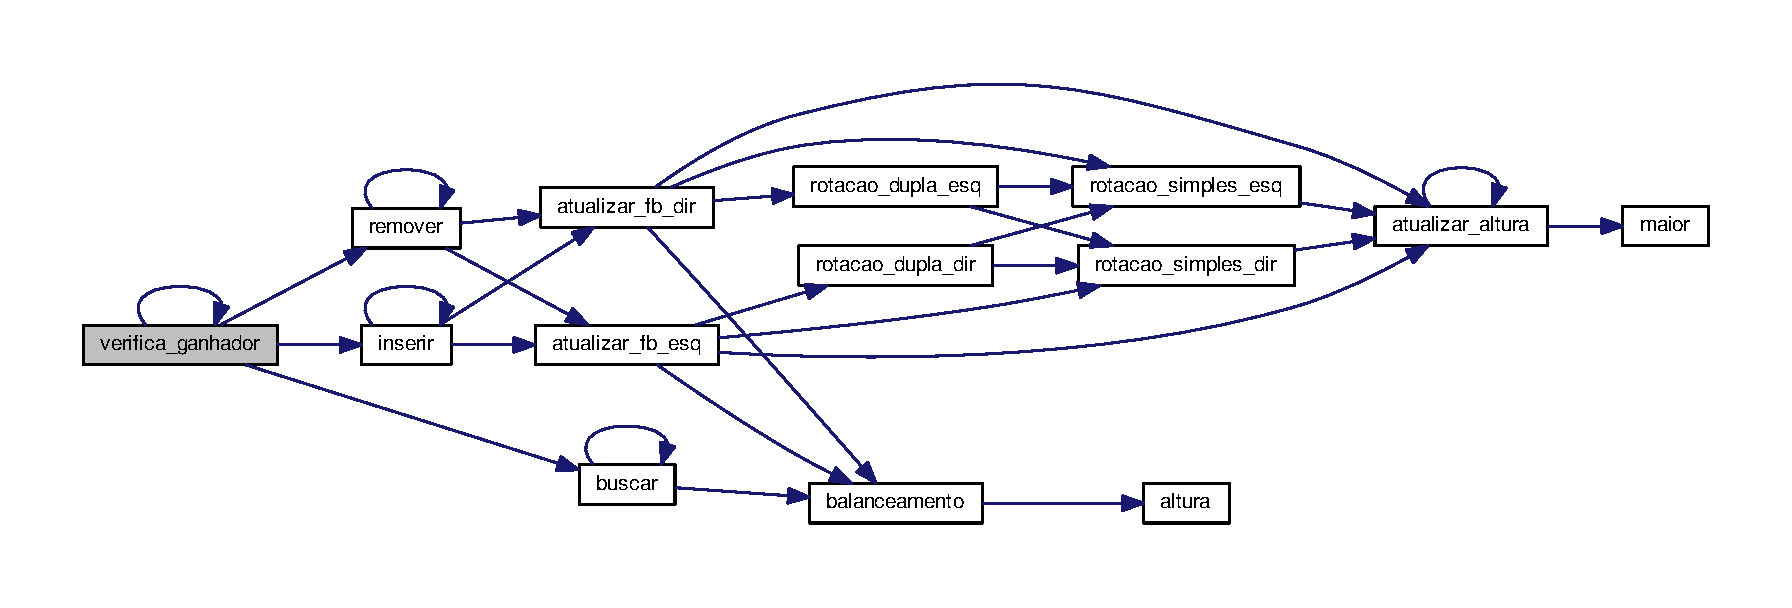
\includegraphics[width=350pt]{avl__jogo__da__velha_8c_a03c14608eb7cb557075be88d2a193e49_cgraph}
\end{center}
\end{figure}




Here is the caller graph for this function\+:
\nopagebreak
\begin{figure}[H]
\begin{center}
\leavevmode
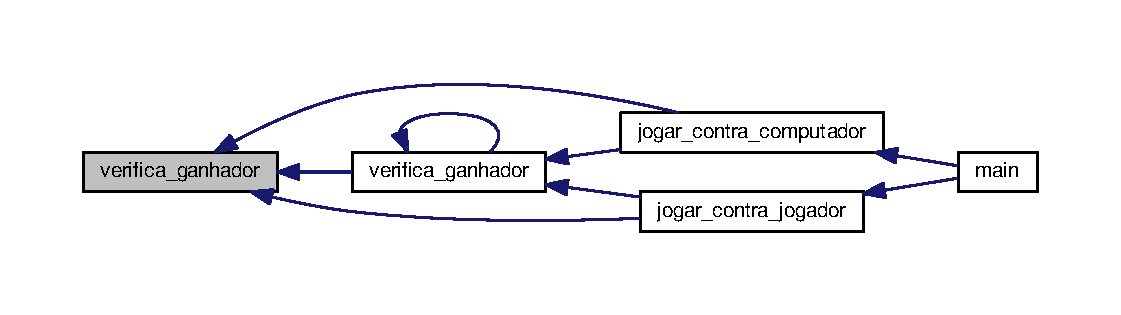
\includegraphics[width=350pt]{avl__jogo__da__velha_8c_a03c14608eb7cb557075be88d2a193e49_icgraph}
\end{center}
\end{figure}



\hypertarget{avl__jogo__da__velha_8h}{}\section{avl\+\_\+jogo\+\_\+da\+\_\+velha.\+h File Reference}
\label{avl__jogo__da__velha_8h}\index{avl\+\_\+jogo\+\_\+da\+\_\+velha.\+h@{avl\+\_\+jogo\+\_\+da\+\_\+velha.\+h}}


É uma biblioteca para manipulação de A\+VL.  


{\ttfamily \#include $<$stdio.\+h$>$}\\*
{\ttfamily \#include $<$stdlib.\+h$>$}\\*
Include dependency graph for avl\+\_\+jogo\+\_\+da\+\_\+velha.\+h\+:\nopagebreak
\begin{figure}[H]
\begin{center}
\leavevmode
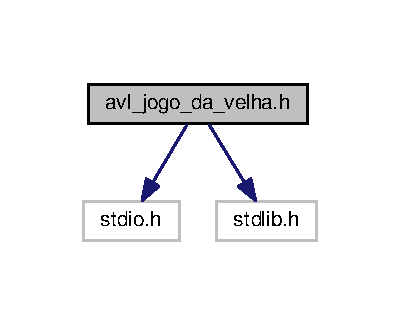
\includegraphics[width=192pt]{avl__jogo__da__velha_8h__incl}
\end{center}
\end{figure}
This graph shows which files directly or indirectly include this file\+:
\nopagebreak
\begin{figure}[H]
\begin{center}
\leavevmode
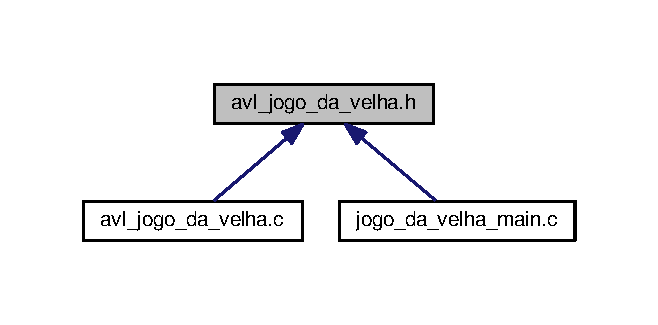
\includegraphics[width=316pt]{avl__jogo__da__velha_8h__dep__incl}
\end{center}
\end{figure}
\subsection*{Data Structures}
\begin{DoxyCompactItemize}
\item 
struct \hyperlink{structnode}{node}
\end{DoxyCompactItemize}
\subsection*{Typedefs}
\begin{DoxyCompactItemize}
\item 
typedef \hyperlink{structstruct}{struct} \hyperlink{structnode}{node} {\bfseries No}\hypertarget{avl__jogo__da__velha_8h_a5e08ad18b152d7695ac344013557a3b5}{}\label{avl__jogo__da__velha_8h_a5e08ad18b152d7695ac344013557a3b5}

\item 
typedef \hyperlink{structstruct}{struct} \hyperlink{structnode}{node} {\bfseries Arvore}\hypertarget{avl__jogo__da__velha_8h_ae211cbdf94cb361e981beeff463707ad}{}\label{avl__jogo__da__velha_8h_ae211cbdf94cb361e981beeff463707ad}

\end{DoxyCompactItemize}
\subsection*{Functions}
\begin{DoxyCompactItemize}
\item 
int \hyperlink{avl__jogo__da__velha_8h_a95df9e1867414fc6300bba61acbea2dc}{maior} (int esq, int dir)
\begin{DoxyCompactList}\small\item\em Função que ao receber 2 inteiro, retorna o maior deles. \end{DoxyCompactList}\item 
int \hyperlink{avl__jogo__da__velha_8h_ac6bb8a4fc7472c16f5f758a7f7425f68}{altura} (\hyperlink{structnode}{Arvore} $\ast$a)
\begin{DoxyCompactList}\small\item\em Função retorna a altura de uma árvore. \end{DoxyCompactList}\item 
int \hyperlink{avl__jogo__da__velha_8h_a7ee46e52a150b1b20c07acb89bf91eff}{atualizar\+\_\+altura} (\hyperlink{structnode}{Arvore} $\ast$a)
\begin{DoxyCompactList}\small\item\em Função recursiva que atualiza as altura da árvore. \end{DoxyCompactList}\item 
int \hyperlink{avl__jogo__da__velha_8h_aa7d437fe01057d6ba284149c0da2eb05}{balanceamento} (\hyperlink{structnode}{Arvore} $\ast$a)
\begin{DoxyCompactList}\small\item\em Função que retorna a diferença das alturas do nós. \end{DoxyCompactList}\item 
\hyperlink{structnode}{Arvore} $\ast$ \hyperlink{avl__jogo__da__velha_8h_a00c2ed93fc83b1c9544215ec43bcbe3b}{rotacao\+\_\+simples\+\_\+esq} (\hyperlink{structnode}{Arvore} $\ast$r)
\begin{DoxyCompactList}\small\item\em Função que realiza uma rotação simples a esquerda na A\+VL. \end{DoxyCompactList}\item 
\hyperlink{structnode}{Arvore} $\ast$ \hyperlink{avl__jogo__da__velha_8h_a4a67cc3736a8b5dcf97b381acd31b367}{rotacao\+\_\+simples\+\_\+dir} (\hyperlink{structnode}{Arvore} $\ast$r)
\begin{DoxyCompactList}\small\item\em Função que realiza uma rotação simples a direita na A\+VL. \end{DoxyCompactList}\item 
\hyperlink{structnode}{Arvore} $\ast$ \hyperlink{avl__jogo__da__velha_8h_acf3488b3e533013675f54b3a7a41817b}{rotacao\+\_\+dupla\+\_\+esq} (\hyperlink{structnode}{Arvore} $\ast$r)
\begin{DoxyCompactList}\small\item\em Função que realiza uma rotação dupla a esquerda na A\+VL. \end{DoxyCompactList}\item 
\hyperlink{structnode}{Arvore} $\ast$ \hyperlink{avl__jogo__da__velha_8h_a75c87c43b3999c5fd0c25bb02dd76236}{rotacao\+\_\+dupla\+\_\+dir} (\hyperlink{structnode}{Arvore} $\ast$r)
\begin{DoxyCompactList}\small\item\em Função que realiza uma rotação dupla a direita na A\+VL. \end{DoxyCompactList}\item 
\hyperlink{structnode}{Arvore} $\ast$ \hyperlink{avl__jogo__da__velha_8h_a2e24e439b994c4a16d861ae3a6614582}{atualizar\+\_\+fb\+\_\+dir} (\hyperlink{structnode}{Arvore} $\ast$r)
\item 
\hyperlink{structnode}{Arvore} $\ast$ \hyperlink{avl__jogo__da__velha_8h_a2e7777768fb10fdf687039c5ebf1116c}{atualizar\+\_\+fb\+\_\+esq} (\hyperlink{structnode}{Arvore} $\ast$r)
\item 
\hyperlink{structnode}{Arvore} $\ast$ \hyperlink{avl__jogo__da__velha_8h_afe18d556ac35160889384a7d7b040248}{inserir} (\hyperlink{structnode}{Arvore} $\ast$a, int chave, int jogador)
\begin{DoxyCompactList}\small\item\em Insere um novo nó na ávore A\+VL. \end{DoxyCompactList}\item 
\hyperlink{structnode}{Arvore} $\ast$ \hyperlink{avl__jogo__da__velha_8h_a265a5bc7a5b7ebc270a8856f54488d03}{remover} (\hyperlink{structnode}{Arvore} $\ast$a, int chave)
\begin{DoxyCompactList}\small\item\em Remove um nó da árvore A\+VL baseado na sua chave. \end{DoxyCompactList}\item 
int \hyperlink{avl__jogo__da__velha_8h_a7554598a42d11e8a4fef8f92c36fe13b}{buscar} (\hyperlink{structnode}{Arvore} $\ast$a, int chave)
\begin{DoxyCompactList}\small\item\em Função que encontra um nó específico baseado em sua chave e retorna o valor da variável jogador. \end{DoxyCompactList}\item 
void {\bfseries imprimir\+\_\+in\+\_\+order} (\hyperlink{structnode}{Arvore} $\ast$a, int nivel)\hypertarget{avl__jogo__da__velha_8h_aea57306782b2e4e71a6d3302c221d59f}{}\label{avl__jogo__da__velha_8h_aea57306782b2e4e71a6d3302c221d59f}

\item 
void {\bfseries arvore\+\_\+para\+\_\+vetor} (\hyperlink{structnode}{Arvore} $\ast$a, int $\ast$tabuleiro)\hypertarget{avl__jogo__da__velha_8h_a2f2c94d4950fc1e1f1e596b0801e1a68}{}\label{avl__jogo__da__velha_8h_a2f2c94d4950fc1e1f1e596b0801e1a68}

\item 
void {\bfseries imprimir\+\_\+tabuleiro} (\hyperlink{structnode}{Arvore} $\ast$a)\hypertarget{avl__jogo__da__velha_8h_a24fd6b104ad2346d6eb7fcab9c68f934}{}\label{avl__jogo__da__velha_8h_a24fd6b104ad2346d6eb7fcab9c68f934}

\item 
int \hyperlink{avl__jogo__da__velha_8h_a03c14608eb7cb557075be88d2a193e49}{verifica\+\_\+ganhador} (\hyperlink{structnode}{Arvore} $\ast$a, int jogador)
\begin{DoxyCompactList}\small\item\em Essa função verifica se alguém ganhou o jogo e retorna um inteiro. \end{DoxyCompactList}\item 
int {\bfseries conta\+\_\+nos} (\hyperlink{structnode}{Arvore} $\ast$a)\hypertarget{avl__jogo__da__velha_8h_ad0e19b40f3c84582310a9e7b64d04ed8}{}\label{avl__jogo__da__velha_8h_ad0e19b40f3c84582310a9e7b64d04ed8}

\item 
void {\bfseries calcula\+\_\+passos} (\hyperlink{structnode}{Arvore} $\ast$$\ast$verificacao, \hyperlink{structnode}{Arvore} $\ast$a, \hyperlink{structnode}{Arvore} $\ast$b, int $\ast$passos, int index)\hypertarget{avl__jogo__da__velha_8h_ad6e0af1d45e4f96223f6423c9221faea}{}\label{avl__jogo__da__velha_8h_ad6e0af1d45e4f96223f6423c9221faea}

\item 
\hyperlink{structnode}{Arvore} $\ast$ {\bfseries jogada\+\_\+computador} (\hyperlink{structnode}{Arvore} $\ast$a, \hyperlink{structnode}{Arvore} $\ast$verificacao)\hypertarget{avl__jogo__da__velha_8h_aa30ea74ebd0880f8e2ca5f9857689b9e}{}\label{avl__jogo__da__velha_8h_aa30ea74ebd0880f8e2ca5f9857689b9e}

\item 
int {\bfseries jogada\+\_\+jogador} ()\hypertarget{avl__jogo__da__velha_8h_a5a10ae88f16cca53770a042c5349697f}{}\label{avl__jogo__da__velha_8h_a5a10ae88f16cca53770a042c5349697f}

\item 
int {\bfseries menu\+\_\+principal} ()\hypertarget{avl__jogo__da__velha_8h_a82bec0e1cbde8c596c089e22096c2092}{}\label{avl__jogo__da__velha_8h_a82bec0e1cbde8c596c089e22096c2092}

\end{DoxyCompactItemize}


\subsection{Detailed Description}
É uma biblioteca para manipulação de A\+VL. 

Essa biblioteca para manipulação de uma A\+VL especial que guarda e gerência dados para o funcionamento do jogo da velha. \begin{DoxyAuthor}{Author}
Lucas Ribeiro 
\end{DoxyAuthor}
\begin{DoxyDate}{Date}
25/05/2017 
\end{DoxyDate}


\subsection{Function Documentation}
\index{avl\+\_\+jogo\+\_\+da\+\_\+velha.\+h@{avl\+\_\+jogo\+\_\+da\+\_\+velha.\+h}!altura@{altura}}
\index{altura@{altura}!avl\+\_\+jogo\+\_\+da\+\_\+velha.\+h@{avl\+\_\+jogo\+\_\+da\+\_\+velha.\+h}}
\subsubsection[{\texorpdfstring{altura(\+Arvore $\ast$a)}{altura(Arvore *a)}}]{\setlength{\rightskip}{0pt plus 5cm}int altura (
\begin{DoxyParamCaption}
\item[{{\bf Arvore} $\ast$}]{a}
\end{DoxyParamCaption}
)}\hypertarget{avl__jogo__da__velha_8h_ac6bb8a4fc7472c16f5f758a7f7425f68}{}\label{avl__jogo__da__velha_8h_ac6bb8a4fc7472c16f5f758a7f7425f68}


Função retorna a altura de uma árvore. 

\begin{DoxyPrecond}{Precondition}
O ponteiro para a árvore não deve ter valor N\+U\+LL 
\end{DoxyPrecond}
\begin{DoxyWarning}{Warning}
Caso o pré requisito não seja atendito a funão retornará N\+U\+LL 
\end{DoxyWarning}

\begin{DoxyParams}{Parameters}
{\em a} & Ponteiro que aponta para a árvore A\+VL. \\
\hline
\end{DoxyParams}
\begin{DoxyReturn}{Returns}
Retorna um inteiro que representa 
\end{DoxyReturn}


Here is the caller graph for this function\+:
\nopagebreak
\begin{figure}[H]
\begin{center}
\leavevmode
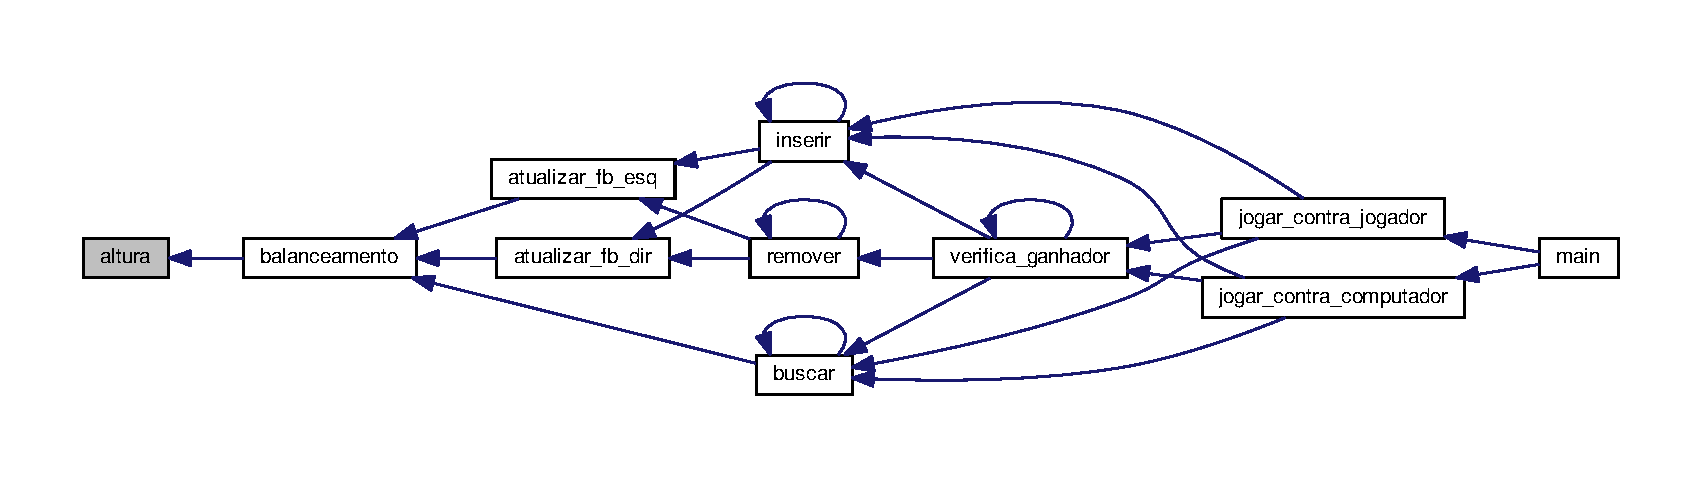
\includegraphics[width=350pt]{avl__jogo__da__velha_8h_ac6bb8a4fc7472c16f5f758a7f7425f68_icgraph}
\end{center}
\end{figure}


\index{avl\+\_\+jogo\+\_\+da\+\_\+velha.\+h@{avl\+\_\+jogo\+\_\+da\+\_\+velha.\+h}!atualizar\+\_\+altura@{atualizar\+\_\+altura}}
\index{atualizar\+\_\+altura@{atualizar\+\_\+altura}!avl\+\_\+jogo\+\_\+da\+\_\+velha.\+h@{avl\+\_\+jogo\+\_\+da\+\_\+velha.\+h}}
\subsubsection[{\texorpdfstring{atualizar\+\_\+altura(\+Arvore $\ast$a)}{atualizar_altura(Arvore *a)}}]{\setlength{\rightskip}{0pt plus 5cm}int atualizar\+\_\+altura (
\begin{DoxyParamCaption}
\item[{{\bf Arvore} $\ast$}]{a}
\end{DoxyParamCaption}
)}\hypertarget{avl__jogo__da__velha_8h_a7ee46e52a150b1b20c07acb89bf91eff}{}\label{avl__jogo__da__velha_8h_a7ee46e52a150b1b20c07acb89bf91eff}


Função recursiva que atualiza as altura da árvore. 


\begin{DoxyParams}{Parameters}
{\em a} & Ponteiro que aponta para o início da A\+VL \\
\hline
\end{DoxyParams}
\begin{DoxyReturn}{Returns}
O retorno inteiro serve para o funcionamento da recursividade. 
\end{DoxyReturn}


Here is the call graph for this function\+:\nopagebreak
\begin{figure}[H]
\begin{center}
\leavevmode
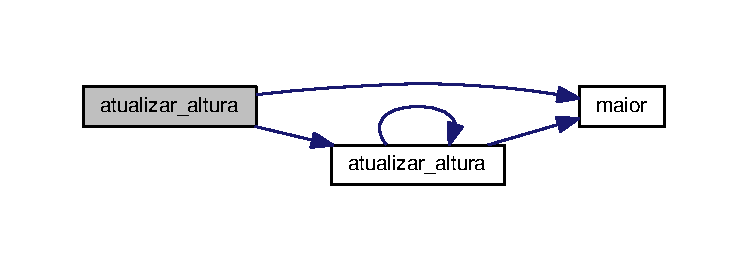
\includegraphics[width=350pt]{avl__jogo__da__velha_8h_a7ee46e52a150b1b20c07acb89bf91eff_cgraph}
\end{center}
\end{figure}




Here is the caller graph for this function\+:
\nopagebreak
\begin{figure}[H]
\begin{center}
\leavevmode
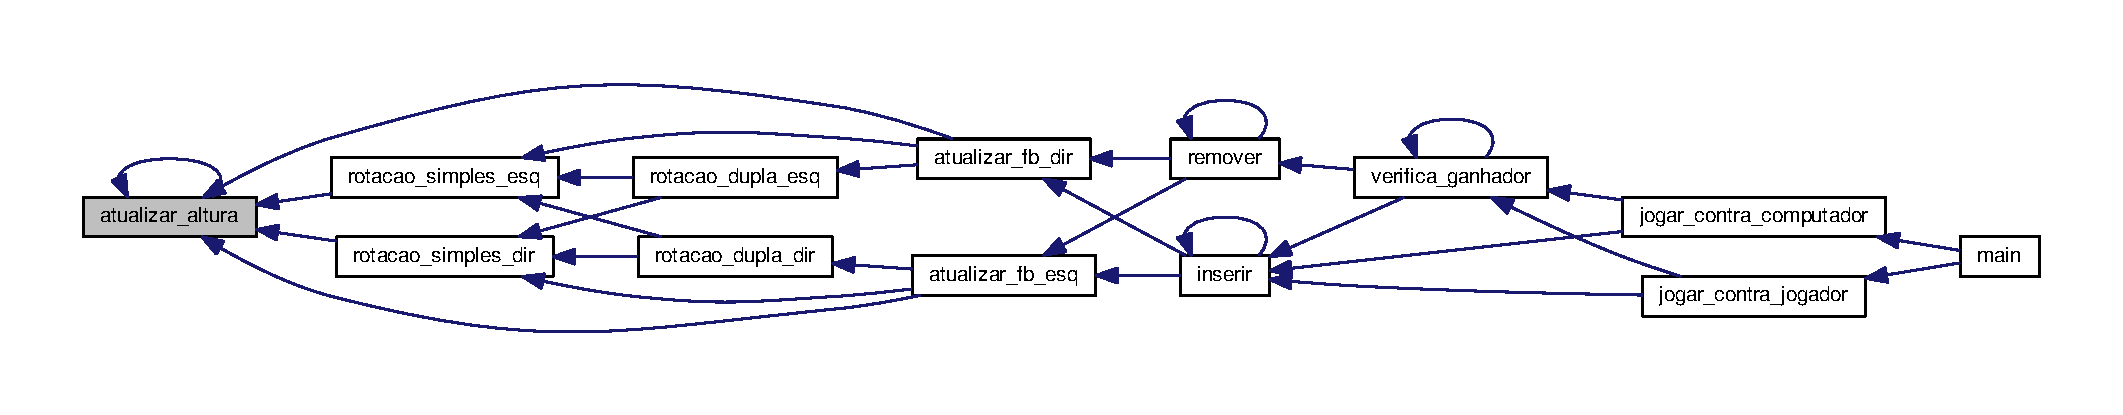
\includegraphics[width=350pt]{avl__jogo__da__velha_8h_a7ee46e52a150b1b20c07acb89bf91eff_icgraph}
\end{center}
\end{figure}


\index{avl\+\_\+jogo\+\_\+da\+\_\+velha.\+h@{avl\+\_\+jogo\+\_\+da\+\_\+velha.\+h}!atualizar\+\_\+fb\+\_\+dir@{atualizar\+\_\+fb\+\_\+dir}}
\index{atualizar\+\_\+fb\+\_\+dir@{atualizar\+\_\+fb\+\_\+dir}!avl\+\_\+jogo\+\_\+da\+\_\+velha.\+h@{avl\+\_\+jogo\+\_\+da\+\_\+velha.\+h}}
\subsubsection[{\texorpdfstring{atualizar\+\_\+fb\+\_\+dir(\+Arvore $\ast$r)}{atualizar_fb_dir(Arvore *r)}}]{\setlength{\rightskip}{0pt plus 5cm}{\bf Arvore}$\ast$ atualizar\+\_\+fb\+\_\+dir (
\begin{DoxyParamCaption}
\item[{{\bf Arvore} $\ast$}]{r}
\end{DoxyParamCaption}
)}\hypertarget{avl__jogo__da__velha_8h_a2e24e439b994c4a16d861ae3a6614582}{}\label{avl__jogo__da__velha_8h_a2e24e439b994c4a16d861ae3a6614582}
Função que atualiza a altura e faz o balanceamento dos nós casos os dá direita estejam desbalanceados. 
\begin{DoxyParams}{Parameters}
{\em r} & Ponteiro que aponta para um nó da árvore A\+VL. \\
\hline
\end{DoxyParams}
\begin{DoxyReturn}{Returns}
Retorna o ponteiro para o nó após as devidas atualizações. 
\end{DoxyReturn}


Here is the call graph for this function\+:\nopagebreak
\begin{figure}[H]
\begin{center}
\leavevmode
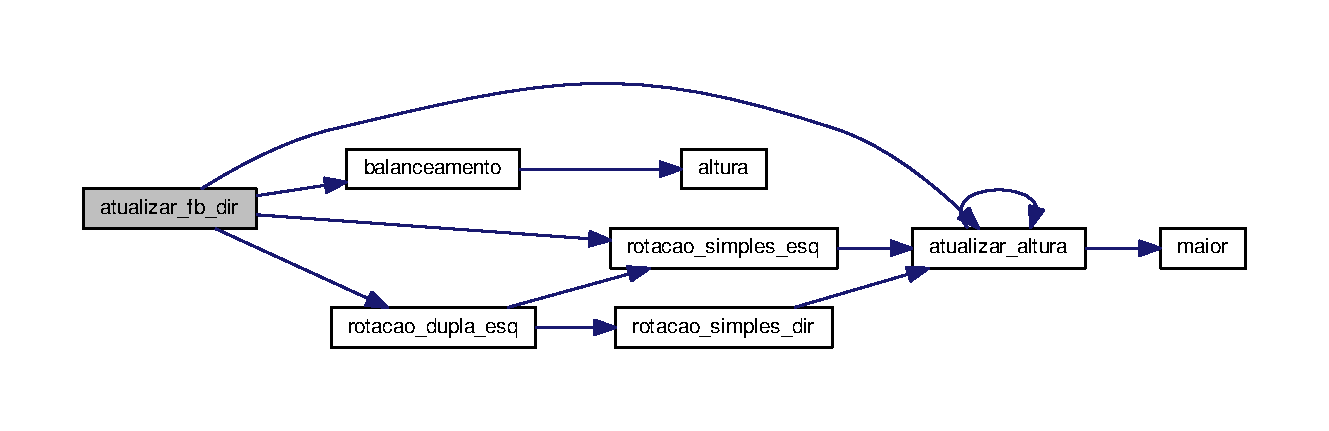
\includegraphics[width=350pt]{avl__jogo__da__velha_8h_a2e24e439b994c4a16d861ae3a6614582_cgraph}
\end{center}
\end{figure}




Here is the caller graph for this function\+:
\nopagebreak
\begin{figure}[H]
\begin{center}
\leavevmode
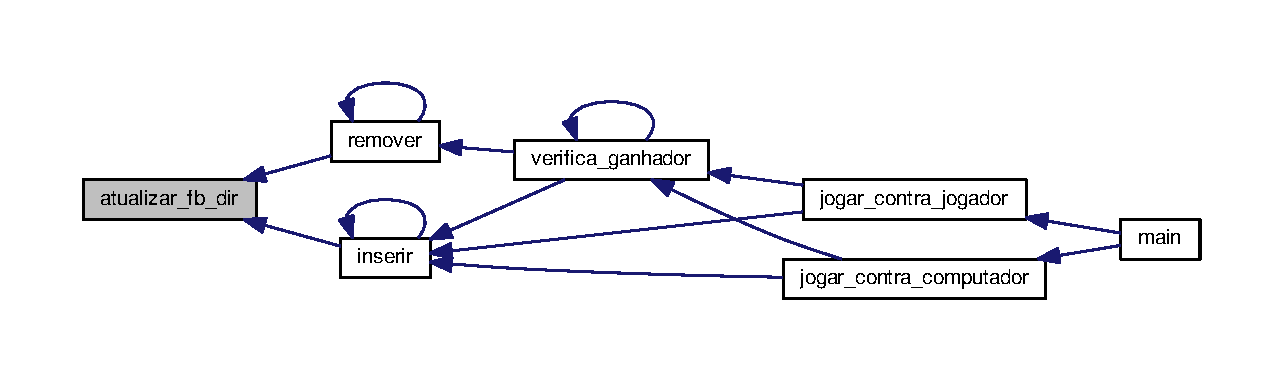
\includegraphics[width=350pt]{avl__jogo__da__velha_8h_a2e24e439b994c4a16d861ae3a6614582_icgraph}
\end{center}
\end{figure}


\index{avl\+\_\+jogo\+\_\+da\+\_\+velha.\+h@{avl\+\_\+jogo\+\_\+da\+\_\+velha.\+h}!atualizar\+\_\+fb\+\_\+esq@{atualizar\+\_\+fb\+\_\+esq}}
\index{atualizar\+\_\+fb\+\_\+esq@{atualizar\+\_\+fb\+\_\+esq}!avl\+\_\+jogo\+\_\+da\+\_\+velha.\+h@{avl\+\_\+jogo\+\_\+da\+\_\+velha.\+h}}
\subsubsection[{\texorpdfstring{atualizar\+\_\+fb\+\_\+esq(\+Arvore $\ast$r)}{atualizar_fb_esq(Arvore *r)}}]{\setlength{\rightskip}{0pt plus 5cm}{\bf Arvore}$\ast$ atualizar\+\_\+fb\+\_\+esq (
\begin{DoxyParamCaption}
\item[{{\bf Arvore} $\ast$}]{r}
\end{DoxyParamCaption}
)}\hypertarget{avl__jogo__da__velha_8h_a2e7777768fb10fdf687039c5ebf1116c}{}\label{avl__jogo__da__velha_8h_a2e7777768fb10fdf687039c5ebf1116c}
Função que atualiza a altura e faz o balancemanto dos nós casos os daá esquerda estejam desbalanceados. 
\begin{DoxyParams}{Parameters}
{\em r} & Ponteiro que aponta para um nó da árvore A\+VL. \\
\hline
\end{DoxyParams}
\begin{DoxyReturn}{Returns}
Retorna o ponteiro para o nó após as devidas alterações feitas. 
\end{DoxyReturn}


Here is the call graph for this function\+:\nopagebreak
\begin{figure}[H]
\begin{center}
\leavevmode
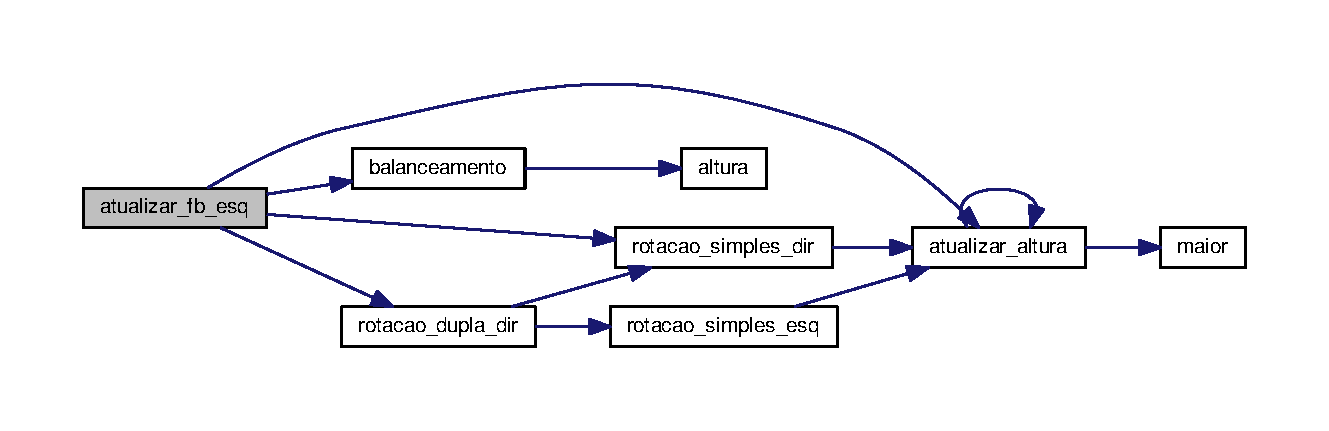
\includegraphics[width=350pt]{avl__jogo__da__velha_8h_a2e7777768fb10fdf687039c5ebf1116c_cgraph}
\end{center}
\end{figure}




Here is the caller graph for this function\+:
\nopagebreak
\begin{figure}[H]
\begin{center}
\leavevmode
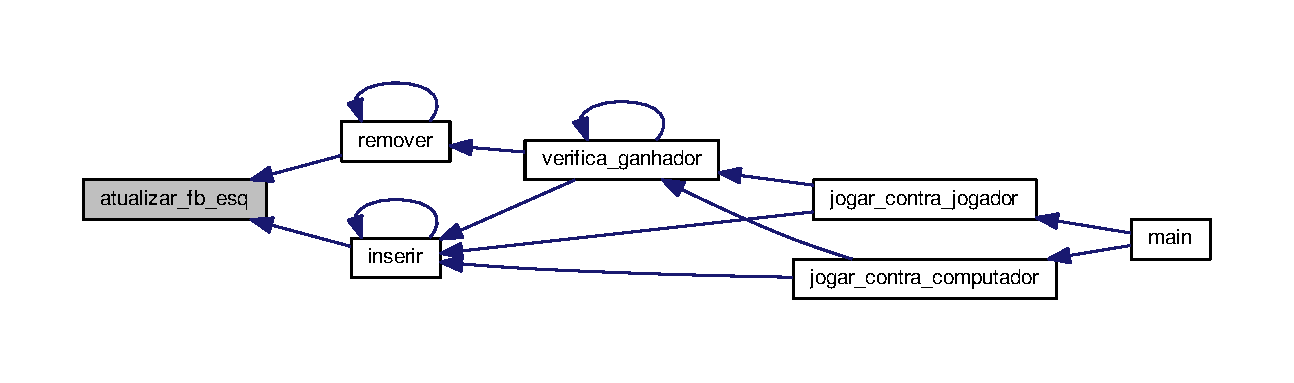
\includegraphics[width=350pt]{avl__jogo__da__velha_8h_a2e7777768fb10fdf687039c5ebf1116c_icgraph}
\end{center}
\end{figure}


\index{avl\+\_\+jogo\+\_\+da\+\_\+velha.\+h@{avl\+\_\+jogo\+\_\+da\+\_\+velha.\+h}!balanceamento@{balanceamento}}
\index{balanceamento@{balanceamento}!avl\+\_\+jogo\+\_\+da\+\_\+velha.\+h@{avl\+\_\+jogo\+\_\+da\+\_\+velha.\+h}}
\subsubsection[{\texorpdfstring{balanceamento(\+Arvore $\ast$a)}{balanceamento(Arvore *a)}}]{\setlength{\rightskip}{0pt plus 5cm}int balanceamento (
\begin{DoxyParamCaption}
\item[{{\bf Arvore} $\ast$}]{a}
\end{DoxyParamCaption}
)}\hypertarget{avl__jogo__da__velha_8h_aa7d437fe01057d6ba284149c0da2eb05}{}\label{avl__jogo__da__velha_8h_aa7d437fe01057d6ba284149c0da2eb05}


Função que retorna a diferença das alturas do nós. 

A função de balancemanto serve para retornar um valor que indica se o nó está balanceado ou não, retornando um valor que vária de -\/2 a 2. 
\begin{DoxyParams}{Parameters}
{\em a} & Ponteiro que aponta para um nó da árvore A\+VL; \\
\hline
\end{DoxyParams}
\begin{DoxyReturn}{Returns}
Retorna o valor do balanceamento 
\end{DoxyReturn}


Here is the call graph for this function\+:\nopagebreak
\begin{figure}[H]
\begin{center}
\leavevmode
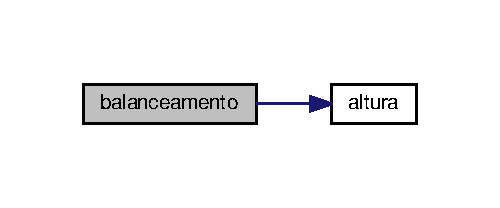
\includegraphics[width=240pt]{avl__jogo__da__velha_8h_aa7d437fe01057d6ba284149c0da2eb05_cgraph}
\end{center}
\end{figure}




Here is the caller graph for this function\+:
\nopagebreak
\begin{figure}[H]
\begin{center}
\leavevmode
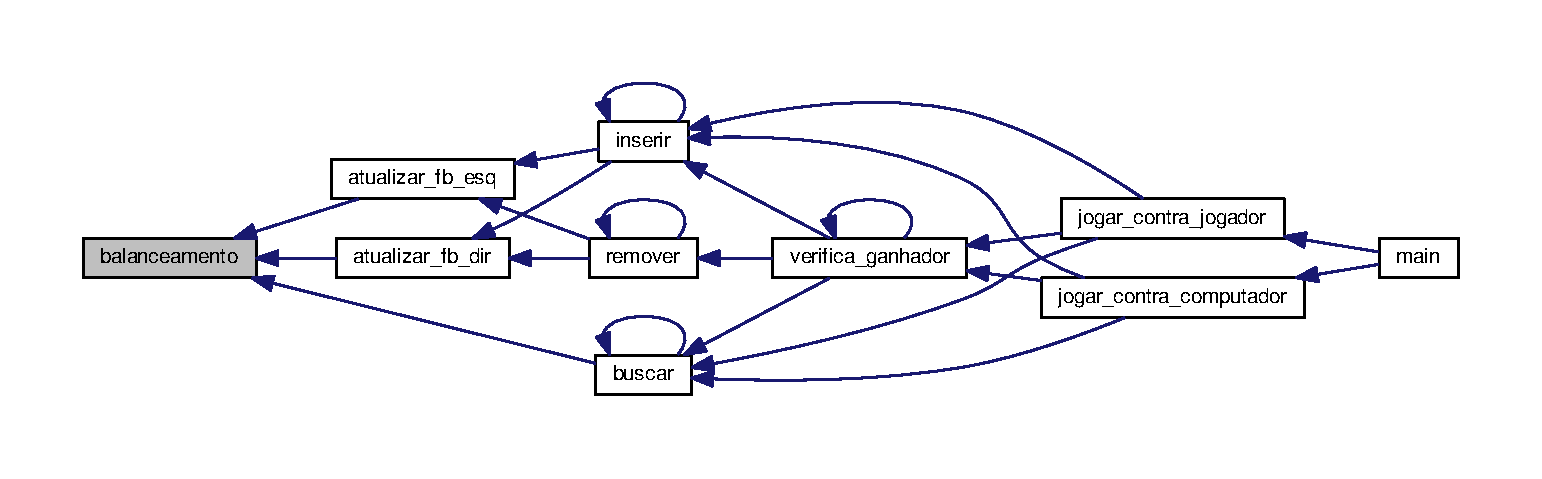
\includegraphics[width=350pt]{avl__jogo__da__velha_8h_aa7d437fe01057d6ba284149c0da2eb05_icgraph}
\end{center}
\end{figure}


\index{avl\+\_\+jogo\+\_\+da\+\_\+velha.\+h@{avl\+\_\+jogo\+\_\+da\+\_\+velha.\+h}!buscar@{buscar}}
\index{buscar@{buscar}!avl\+\_\+jogo\+\_\+da\+\_\+velha.\+h@{avl\+\_\+jogo\+\_\+da\+\_\+velha.\+h}}
\subsubsection[{\texorpdfstring{buscar(\+Arvore $\ast$a, int chave)}{buscar(Arvore *a, int chave)}}]{\setlength{\rightskip}{0pt plus 5cm}int buscar (
\begin{DoxyParamCaption}
\item[{{\bf Arvore} $\ast$}]{a, }
\item[{int}]{chave}
\end{DoxyParamCaption}
)}\hypertarget{avl__jogo__da__velha_8h_a7554598a42d11e8a4fef8f92c36fe13b}{}\label{avl__jogo__da__velha_8h_a7554598a42d11e8a4fef8f92c36fe13b}


Função que encontra um nó específico baseado em sua chave e retorna o valor da variável jogador. 


\begin{DoxyParams}{Parameters}
{\em a} & Ponteiro que aponta para a ávore em que se deseja buscar. \\
\hline
{\em chave} & Inteiro que representa a chave do nó que se deseja achar. \\
\hline
\end{DoxyParams}
\begin{DoxyReturn}{Returns}
Retorna um inteiro com o mesmo valor da variável jogador do nó que se buscava. 
\end{DoxyReturn}


Here is the call graph for this function\+:\nopagebreak
\begin{figure}[H]
\begin{center}
\leavevmode
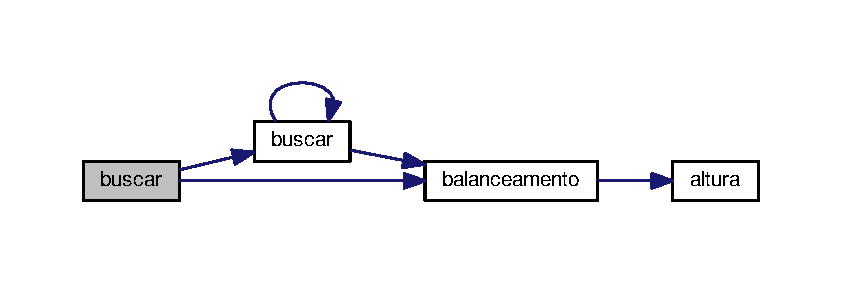
\includegraphics[width=350pt]{avl__jogo__da__velha_8h_a7554598a42d11e8a4fef8f92c36fe13b_cgraph}
\end{center}
\end{figure}




Here is the caller graph for this function\+:
\nopagebreak
\begin{figure}[H]
\begin{center}
\leavevmode
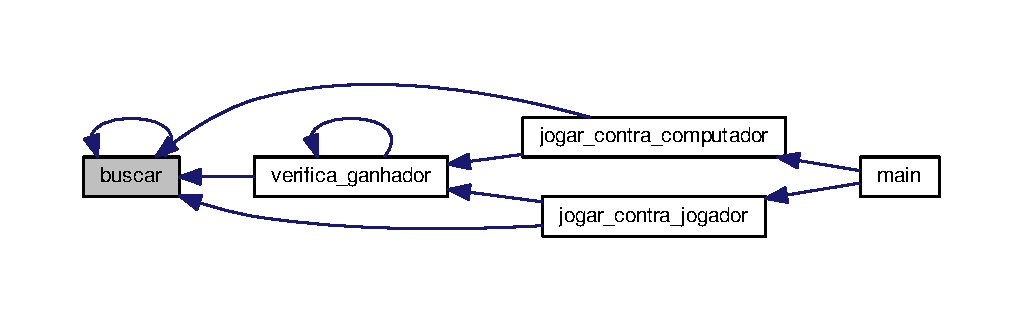
\includegraphics[width=350pt]{avl__jogo__da__velha_8h_a7554598a42d11e8a4fef8f92c36fe13b_icgraph}
\end{center}
\end{figure}


\index{avl\+\_\+jogo\+\_\+da\+\_\+velha.\+h@{avl\+\_\+jogo\+\_\+da\+\_\+velha.\+h}!inserir@{inserir}}
\index{inserir@{inserir}!avl\+\_\+jogo\+\_\+da\+\_\+velha.\+h@{avl\+\_\+jogo\+\_\+da\+\_\+velha.\+h}}
\subsubsection[{\texorpdfstring{inserir(\+Arvore $\ast$a, int chave, int jogador)}{inserir(Arvore *a, int chave, int jogador)}}]{\setlength{\rightskip}{0pt plus 5cm}{\bf Arvore}$\ast$ inserir (
\begin{DoxyParamCaption}
\item[{{\bf Arvore} $\ast$}]{a, }
\item[{int}]{chave, }
\item[{int}]{jogador}
\end{DoxyParamCaption}
)}\hypertarget{avl__jogo__da__velha_8h_afe18d556ac35160889384a7d7b040248}{}\label{avl__jogo__da__velha_8h_afe18d556ac35160889384a7d7b040248}


Insere um novo nó na ávore A\+VL. 


\begin{DoxyParams}{Parameters}
{\em a} & É um ponteiro que representa a árvore onde se quer inserir. \\
\hline
{\em chave} & É um inteiro que representa o valor do nó. \\
\hline
{\em jogador} & É um inteiro que representa o jogador que fez a jogada. \\
\hline
\end{DoxyParams}
\begin{DoxyReturn}{Returns}
Retorna o ponteiro para árvore após a inserção ter sido feita. 
\end{DoxyReturn}


Here is the call graph for this function\+:\nopagebreak
\begin{figure}[H]
\begin{center}
\leavevmode
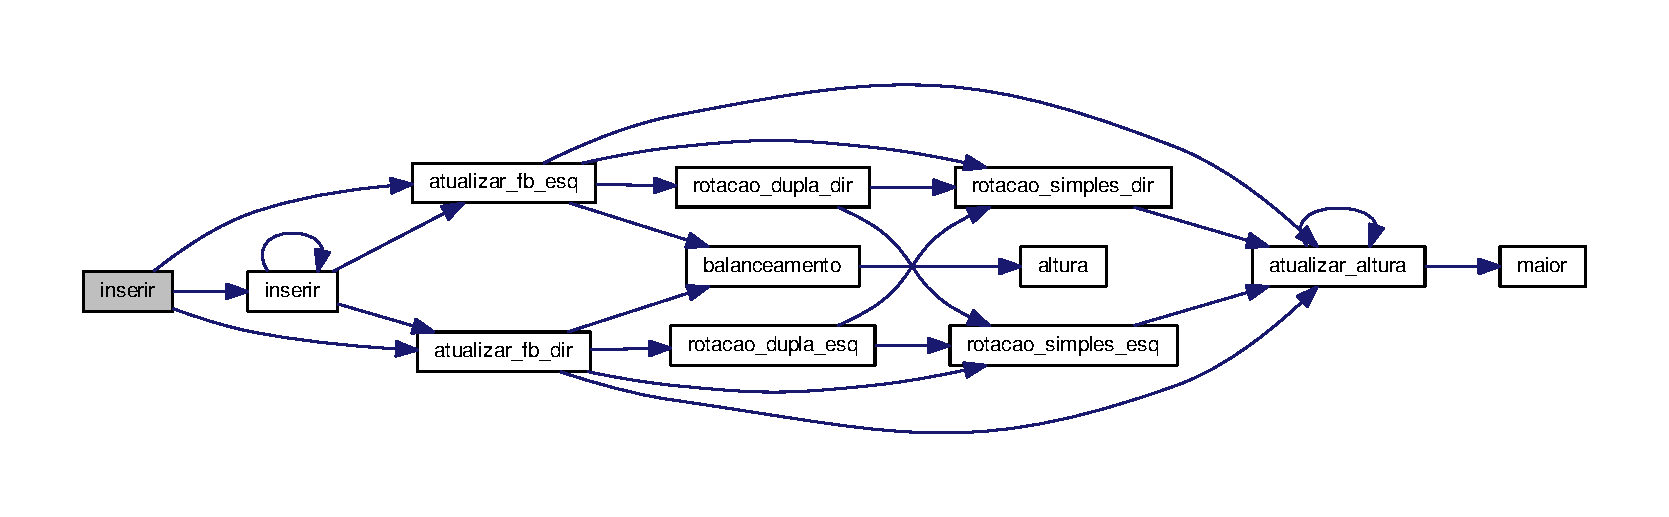
\includegraphics[width=350pt]{avl__jogo__da__velha_8h_afe18d556ac35160889384a7d7b040248_cgraph}
\end{center}
\end{figure}




Here is the caller graph for this function\+:
\nopagebreak
\begin{figure}[H]
\begin{center}
\leavevmode
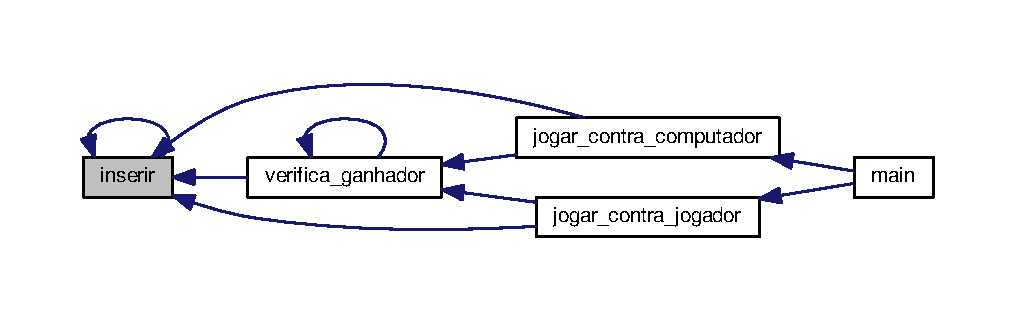
\includegraphics[width=350pt]{avl__jogo__da__velha_8h_afe18d556ac35160889384a7d7b040248_icgraph}
\end{center}
\end{figure}


\index{avl\+\_\+jogo\+\_\+da\+\_\+velha.\+h@{avl\+\_\+jogo\+\_\+da\+\_\+velha.\+h}!maior@{maior}}
\index{maior@{maior}!avl\+\_\+jogo\+\_\+da\+\_\+velha.\+h@{avl\+\_\+jogo\+\_\+da\+\_\+velha.\+h}}
\subsubsection[{\texorpdfstring{maior(int esq, int dir)}{maior(int esq, int dir)}}]{\setlength{\rightskip}{0pt plus 5cm}int maior (
\begin{DoxyParamCaption}
\item[{int}]{esq, }
\item[{int}]{dir}
\end{DoxyParamCaption}
)}\hypertarget{avl__jogo__da__velha_8h_a95df9e1867414fc6300bba61acbea2dc}{}\label{avl__jogo__da__velha_8h_a95df9e1867414fc6300bba61acbea2dc}


Função que ao receber 2 inteiro, retorna o maior deles. 


\begin{DoxyParams}{Parameters}
{\em esq} & Inteiro que representa o valor a esquerda da A\+VL. \\
\hline
{\em dir} & Inteiro que representa o valor a direita da A\+VL. \\
\hline
\end{DoxyParams}
\begin{DoxyReturn}{Returns}
Retorno inteiro que representa o maior de ambos os valores. 
\end{DoxyReturn}


Here is the caller graph for this function\+:
\nopagebreak
\begin{figure}[H]
\begin{center}
\leavevmode
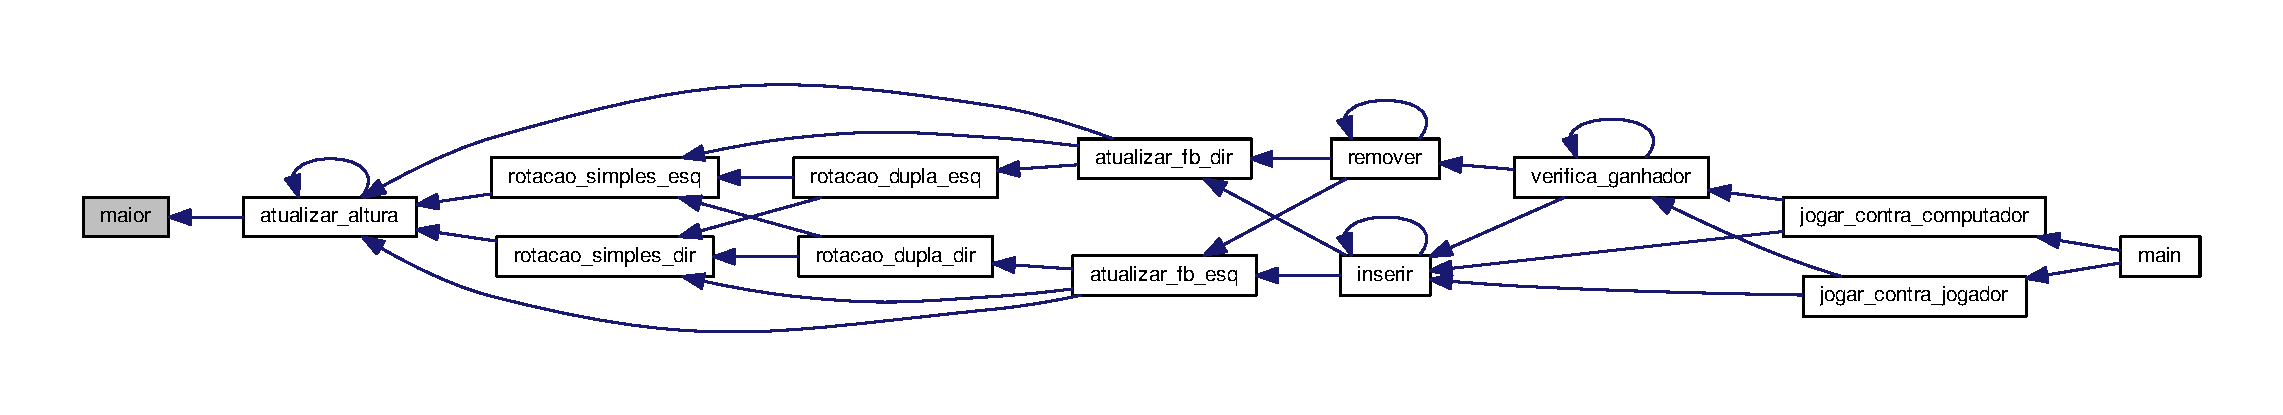
\includegraphics[width=350pt]{avl__jogo__da__velha_8h_a95df9e1867414fc6300bba61acbea2dc_icgraph}
\end{center}
\end{figure}


\index{avl\+\_\+jogo\+\_\+da\+\_\+velha.\+h@{avl\+\_\+jogo\+\_\+da\+\_\+velha.\+h}!remover@{remover}}
\index{remover@{remover}!avl\+\_\+jogo\+\_\+da\+\_\+velha.\+h@{avl\+\_\+jogo\+\_\+da\+\_\+velha.\+h}}
\subsubsection[{\texorpdfstring{remover(\+Arvore $\ast$a, int chave)}{remover(Arvore *a, int chave)}}]{\setlength{\rightskip}{0pt plus 5cm}{\bf Arvore}$\ast$ remover (
\begin{DoxyParamCaption}
\item[{{\bf Arvore} $\ast$}]{a, }
\item[{int}]{chave}
\end{DoxyParamCaption}
)}\hypertarget{avl__jogo__da__velha_8h_a265a5bc7a5b7ebc270a8856f54488d03}{}\label{avl__jogo__da__velha_8h_a265a5bc7a5b7ebc270a8856f54488d03}


Remove um nó da árvore A\+VL baseado na sua chave. 


\begin{DoxyParams}{Parameters}
{\em a} & É um ponteiro que aponta para a árvore ao qual se deseja remover o nó. \\
\hline
{\em chave} & É um inteiro que representa a chave do nó que se pretende remover \\
\hline
\end{DoxyParams}
\begin{DoxyReturn}{Returns}
Retorna o ponteiro para a árvore, após ter sido removido o nó. 
\end{DoxyReturn}


Here is the call graph for this function\+:\nopagebreak
\begin{figure}[H]
\begin{center}
\leavevmode
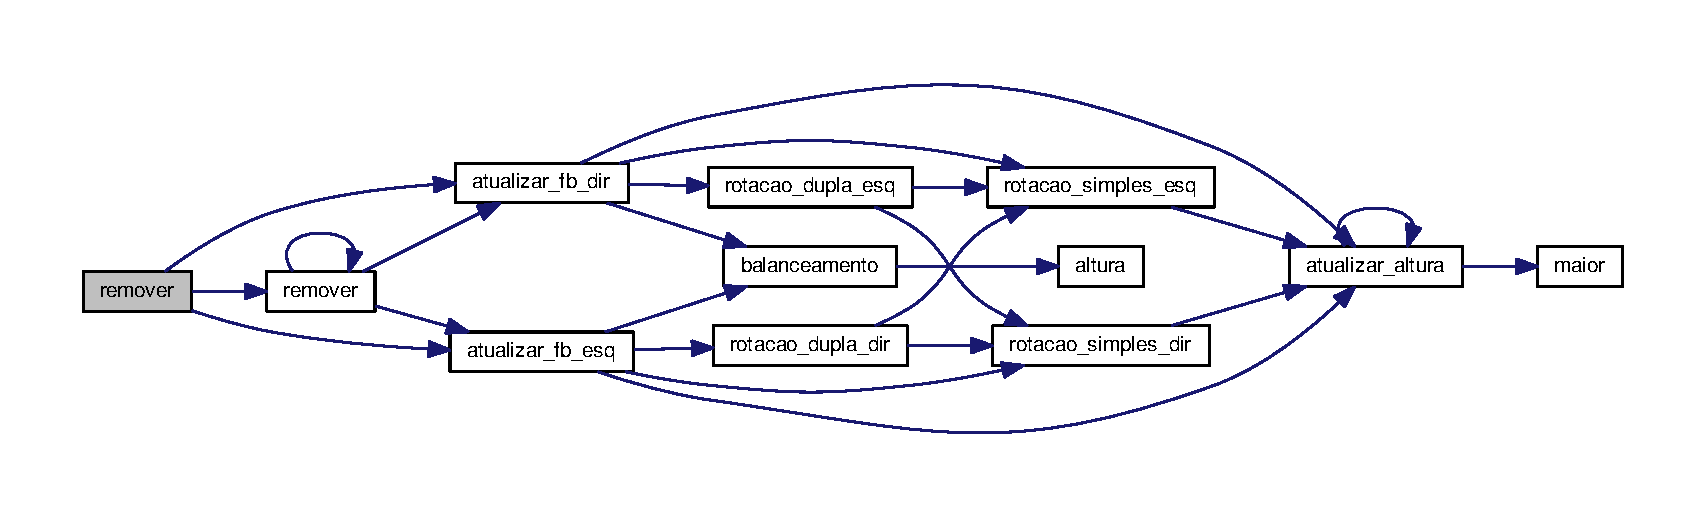
\includegraphics[width=350pt]{avl__jogo__da__velha_8h_a265a5bc7a5b7ebc270a8856f54488d03_cgraph}
\end{center}
\end{figure}




Here is the caller graph for this function\+:
\nopagebreak
\begin{figure}[H]
\begin{center}
\leavevmode
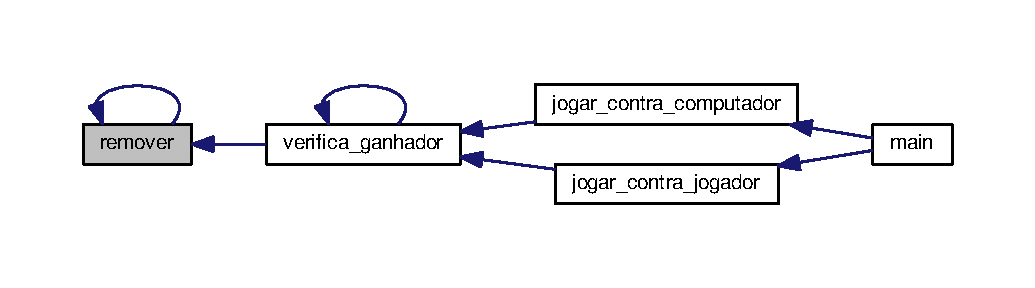
\includegraphics[width=350pt]{avl__jogo__da__velha_8h_a265a5bc7a5b7ebc270a8856f54488d03_icgraph}
\end{center}
\end{figure}


\index{avl\+\_\+jogo\+\_\+da\+\_\+velha.\+h@{avl\+\_\+jogo\+\_\+da\+\_\+velha.\+h}!rotacao\+\_\+dupla\+\_\+dir@{rotacao\+\_\+dupla\+\_\+dir}}
\index{rotacao\+\_\+dupla\+\_\+dir@{rotacao\+\_\+dupla\+\_\+dir}!avl\+\_\+jogo\+\_\+da\+\_\+velha.\+h@{avl\+\_\+jogo\+\_\+da\+\_\+velha.\+h}}
\subsubsection[{\texorpdfstring{rotacao\+\_\+dupla\+\_\+dir(\+Arvore $\ast$r)}{rotacao_dupla_dir(Arvore *r)}}]{\setlength{\rightskip}{0pt plus 5cm}{\bf Arvore}$\ast$ rotacao\+\_\+dupla\+\_\+dir (
\begin{DoxyParamCaption}
\item[{{\bf Arvore} $\ast$}]{r}
\end{DoxyParamCaption}
)}\hypertarget{avl__jogo__da__velha_8h_a75c87c43b3999c5fd0c25bb02dd76236}{}\label{avl__jogo__da__velha_8h_a75c87c43b3999c5fd0c25bb02dd76236}


Função que realiza uma rotação dupla a direita na A\+VL. 


\begin{DoxyParams}{Parameters}
{\em r} & Ponteiro que aponta para um nó da árvore A\+VL. \\
\hline
\end{DoxyParams}
\begin{DoxyReturn}{Returns}
Retorna o ponteiro do nó da A\+VL após a rotação feita. 
\end{DoxyReturn}


Here is the call graph for this function\+:\nopagebreak
\begin{figure}[H]
\begin{center}
\leavevmode
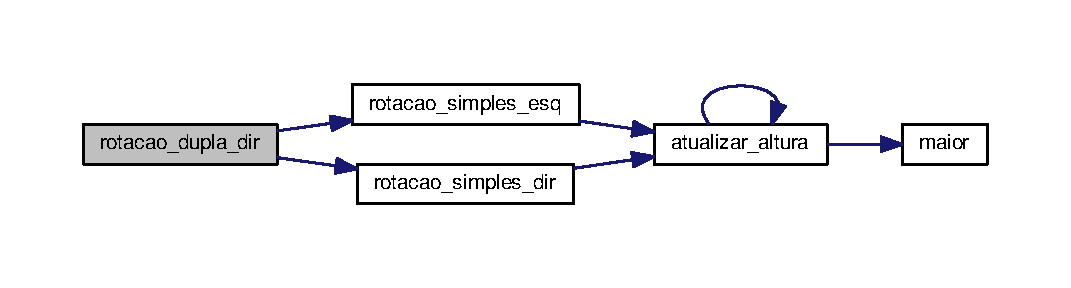
\includegraphics[width=350pt]{avl__jogo__da__velha_8h_a75c87c43b3999c5fd0c25bb02dd76236_cgraph}
\end{center}
\end{figure}




Here is the caller graph for this function\+:
\nopagebreak
\begin{figure}[H]
\begin{center}
\leavevmode
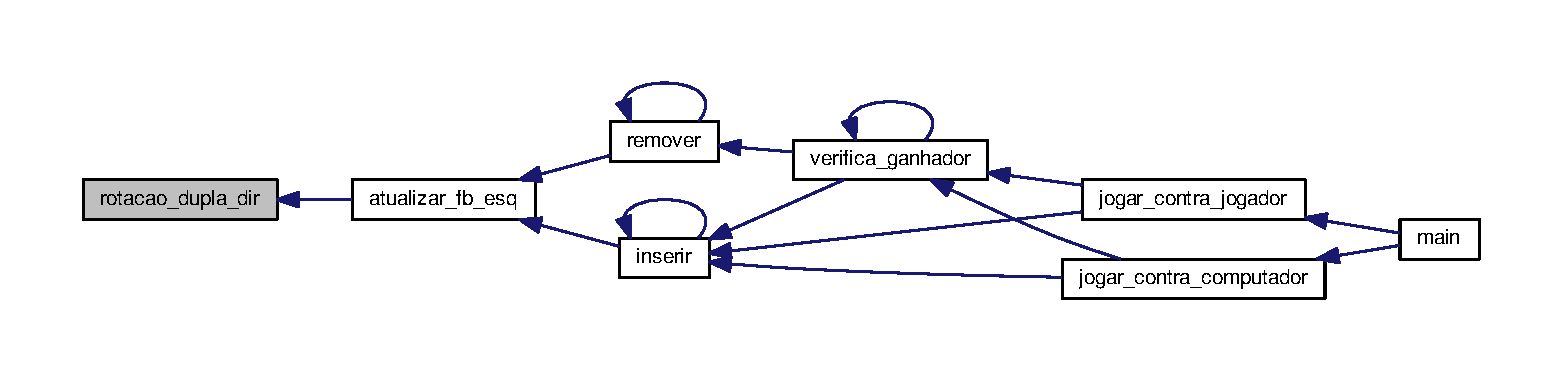
\includegraphics[width=350pt]{avl__jogo__da__velha_8h_a75c87c43b3999c5fd0c25bb02dd76236_icgraph}
\end{center}
\end{figure}


\index{avl\+\_\+jogo\+\_\+da\+\_\+velha.\+h@{avl\+\_\+jogo\+\_\+da\+\_\+velha.\+h}!rotacao\+\_\+dupla\+\_\+esq@{rotacao\+\_\+dupla\+\_\+esq}}
\index{rotacao\+\_\+dupla\+\_\+esq@{rotacao\+\_\+dupla\+\_\+esq}!avl\+\_\+jogo\+\_\+da\+\_\+velha.\+h@{avl\+\_\+jogo\+\_\+da\+\_\+velha.\+h}}
\subsubsection[{\texorpdfstring{rotacao\+\_\+dupla\+\_\+esq(\+Arvore $\ast$r)}{rotacao_dupla_esq(Arvore *r)}}]{\setlength{\rightskip}{0pt plus 5cm}{\bf Arvore}$\ast$ rotacao\+\_\+dupla\+\_\+esq (
\begin{DoxyParamCaption}
\item[{{\bf Arvore} $\ast$}]{r}
\end{DoxyParamCaption}
)}\hypertarget{avl__jogo__da__velha_8h_acf3488b3e533013675f54b3a7a41817b}{}\label{avl__jogo__da__velha_8h_acf3488b3e533013675f54b3a7a41817b}


Função que realiza uma rotação dupla a esquerda na A\+VL. 


\begin{DoxyParams}{Parameters}
{\em r} & Ponteiro que aponta para um nó da árvore A\+VL. \\
\hline
\end{DoxyParams}
\begin{DoxyReturn}{Returns}
Retorna o ponteiro do nó da A\+VL após a rotação feita. 
\end{DoxyReturn}


Here is the call graph for this function\+:\nopagebreak
\begin{figure}[H]
\begin{center}
\leavevmode
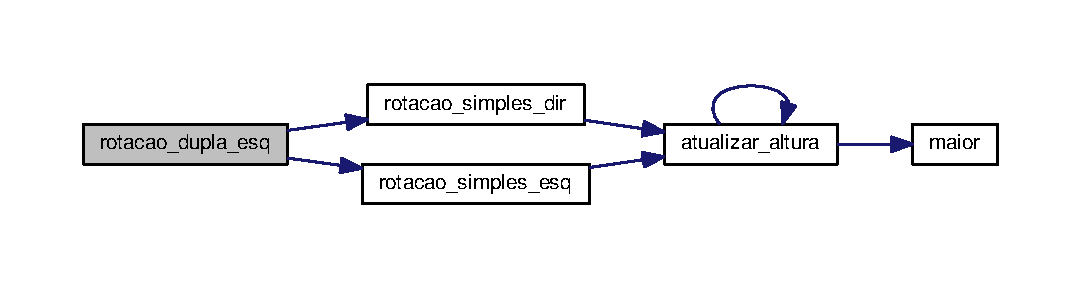
\includegraphics[width=350pt]{avl__jogo__da__velha_8h_acf3488b3e533013675f54b3a7a41817b_cgraph}
\end{center}
\end{figure}




Here is the caller graph for this function\+:
\nopagebreak
\begin{figure}[H]
\begin{center}
\leavevmode
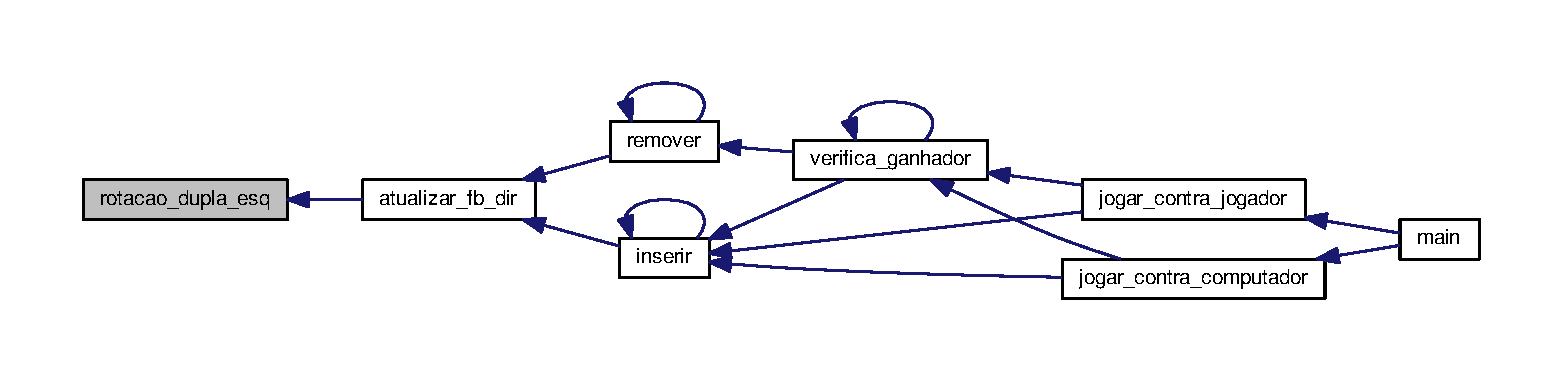
\includegraphics[width=350pt]{avl__jogo__da__velha_8h_acf3488b3e533013675f54b3a7a41817b_icgraph}
\end{center}
\end{figure}


\index{avl\+\_\+jogo\+\_\+da\+\_\+velha.\+h@{avl\+\_\+jogo\+\_\+da\+\_\+velha.\+h}!rotacao\+\_\+simples\+\_\+dir@{rotacao\+\_\+simples\+\_\+dir}}
\index{rotacao\+\_\+simples\+\_\+dir@{rotacao\+\_\+simples\+\_\+dir}!avl\+\_\+jogo\+\_\+da\+\_\+velha.\+h@{avl\+\_\+jogo\+\_\+da\+\_\+velha.\+h}}
\subsubsection[{\texorpdfstring{rotacao\+\_\+simples\+\_\+dir(\+Arvore $\ast$r)}{rotacao_simples_dir(Arvore *r)}}]{\setlength{\rightskip}{0pt plus 5cm}{\bf Arvore}$\ast$ rotacao\+\_\+simples\+\_\+dir (
\begin{DoxyParamCaption}
\item[{{\bf Arvore} $\ast$}]{r}
\end{DoxyParamCaption}
)}\hypertarget{avl__jogo__da__velha_8h_a4a67cc3736a8b5dcf97b381acd31b367}{}\label{avl__jogo__da__velha_8h_a4a67cc3736a8b5dcf97b381acd31b367}


Função que realiza uma rotação simples a direita na A\+VL. 


\begin{DoxyParams}{Parameters}
{\em r} & Ponteiro que aponta para um nó da árvore A\+VL. \\
\hline
\end{DoxyParams}
\begin{DoxyReturn}{Returns}
Retorna o ponteiro do nó da A\+VL após a rotação feita 
\end{DoxyReturn}


Here is the call graph for this function\+:\nopagebreak
\begin{figure}[H]
\begin{center}
\leavevmode
\includegraphics[width=350pt]{avl__jogo__da__velha_8h_a4a67cc3736a8b5dcf97b381acd31b367_cgraph}
\end{center}
\end{figure}




Here is the caller graph for this function\+:
\nopagebreak
\begin{figure}[H]
\begin{center}
\leavevmode
\includegraphics[width=350pt]{avl__jogo__da__velha_8h_a4a67cc3736a8b5dcf97b381acd31b367_icgraph}
\end{center}
\end{figure}


\index{avl\+\_\+jogo\+\_\+da\+\_\+velha.\+h@{avl\+\_\+jogo\+\_\+da\+\_\+velha.\+h}!rotacao\+\_\+simples\+\_\+esq@{rotacao\+\_\+simples\+\_\+esq}}
\index{rotacao\+\_\+simples\+\_\+esq@{rotacao\+\_\+simples\+\_\+esq}!avl\+\_\+jogo\+\_\+da\+\_\+velha.\+h@{avl\+\_\+jogo\+\_\+da\+\_\+velha.\+h}}
\subsubsection[{\texorpdfstring{rotacao\+\_\+simples\+\_\+esq(\+Arvore $\ast$r)}{rotacao_simples_esq(Arvore *r)}}]{\setlength{\rightskip}{0pt plus 5cm}{\bf Arvore}$\ast$ rotacao\+\_\+simples\+\_\+esq (
\begin{DoxyParamCaption}
\item[{{\bf Arvore} $\ast$}]{r}
\end{DoxyParamCaption}
)}\hypertarget{avl__jogo__da__velha_8h_a00c2ed93fc83b1c9544215ec43bcbe3b}{}\label{avl__jogo__da__velha_8h_a00c2ed93fc83b1c9544215ec43bcbe3b}


Função que realiza uma rotação simples a esquerda na A\+VL. 


\begin{DoxyParams}{Parameters}
{\em r} & Ponteiro que aponta para um nó da árvore A\+V\+L! \\
\hline
\end{DoxyParams}
\begin{DoxyReturn}{Returns}
Retorna o ponteiro do nó da A\+VL após a rotação feita 
\end{DoxyReturn}


Here is the call graph for this function\+:\nopagebreak
\begin{figure}[H]
\begin{center}
\leavevmode
\includegraphics[width=350pt]{avl__jogo__da__velha_8h_a00c2ed93fc83b1c9544215ec43bcbe3b_cgraph}
\end{center}
\end{figure}




Here is the caller graph for this function\+:
\nopagebreak
\begin{figure}[H]
\begin{center}
\leavevmode
\includegraphics[width=350pt]{avl__jogo__da__velha_8h_a00c2ed93fc83b1c9544215ec43bcbe3b_icgraph}
\end{center}
\end{figure}


\index{avl\+\_\+jogo\+\_\+da\+\_\+velha.\+h@{avl\+\_\+jogo\+\_\+da\+\_\+velha.\+h}!verifica\+\_\+ganhador@{verifica\+\_\+ganhador}}
\index{verifica\+\_\+ganhador@{verifica\+\_\+ganhador}!avl\+\_\+jogo\+\_\+da\+\_\+velha.\+h@{avl\+\_\+jogo\+\_\+da\+\_\+velha.\+h}}
\subsubsection[{\texorpdfstring{verifica\+\_\+ganhador(\+Arvore $\ast$a, int jogador)}{verifica_ganhador(Arvore *a, int jogador)}}]{\setlength{\rightskip}{0pt plus 5cm}int verifica\+\_\+ganhador (
\begin{DoxyParamCaption}
\item[{{\bf Arvore} $\ast$}]{a, }
\item[{int}]{jogador}
\end{DoxyParamCaption}
)}\hypertarget{avl__jogo__da__velha_8h_a03c14608eb7cb557075be88d2a193e49}{}\label{avl__jogo__da__velha_8h_a03c14608eb7cb557075be88d2a193e49}


Essa função verifica se alguém ganhou o jogo e retorna um inteiro. 


\begin{DoxyParams}{Parameters}
{\em a} & É um ponteiro para a árvore A\+VL. \\
\hline
{\em jogador} & É um inteiro que representa qual jogador se está verificando. \\
\hline
\end{DoxyParams}
\begin{DoxyReturn}{Returns}
Inteiro de retorno 
\end{DoxyReturn}


Here is the call graph for this function\+:\nopagebreak
\begin{figure}[H]
\begin{center}
\leavevmode
\includegraphics[width=350pt]{avl__jogo__da__velha_8h_a03c14608eb7cb557075be88d2a193e49_cgraph}
\end{center}
\end{figure}




Here is the caller graph for this function\+:
\nopagebreak
\begin{figure}[H]
\begin{center}
\leavevmode
\includegraphics[width=350pt]{avl__jogo__da__velha_8h_a03c14608eb7cb557075be88d2a193e49_icgraph}
\end{center}
\end{figure}



\hypertarget{jogo__da__velha__main_8c}{}\section{jogo\+\_\+da\+\_\+velha\+\_\+main.\+c File Reference}
\label{jogo__da__velha__main_8c}\index{jogo\+\_\+da\+\_\+velha\+\_\+main.\+c@{jogo\+\_\+da\+\_\+velha\+\_\+main.\+c}}


Código fonte do jogo da velha.  


{\ttfamily \#include $<$stdbool.\+h$>$}\\*
{\ttfamily \#include \char`\"{}avl\+\_\+jogo\+\_\+da\+\_\+velha.\+h\char`\"{}}\\*
Include dependency graph for jogo\+\_\+da\+\_\+velha\+\_\+main.\+c\+:
\nopagebreak
\begin{figure}[H]
\begin{center}
\leavevmode
\includegraphics[width=263pt]{jogo__da__velha__main_8c__incl}
\end{center}
\end{figure}
\subsection*{Functions}
\begin{DoxyCompactItemize}
\item 
void \hyperlink{jogo__da__velha__main_8c_a122bc80c1701fe7d714188c3f55197f2}{jogar\+\_\+contra\+\_\+computador} (\hyperlink{structnode}{Arvore} $\ast$a)
\begin{DoxyCompactList}\small\item\em Função que controla o jogo quando selecionado a opção Player vs IA. \end{DoxyCompactList}\item 
void \hyperlink{jogo__da__velha__main_8c_aa24f40cfc3db5d038952a99c9300655b}{jogar\+\_\+contra\+\_\+jogador} (\hyperlink{structnode}{Arvore} $\ast$a)
\begin{DoxyCompactList}\small\item\em Função que controla o jogo quando é selecionado a opção de Player vc Player. \end{DoxyCompactList}\item 
int \hyperlink{jogo__da__velha__main_8c_ae66f6b31b5ad750f1fe042a706a4e3d4}{main} ()
\begin{DoxyCompactList}\small\item\em Função Main do programa C. \end{DoxyCompactList}\end{DoxyCompactItemize}


\subsection{Detailed Description}
Código fonte do jogo da velha. 

\begin{DoxyAuthor}{Author}
Lucas Ribeiro 
\end{DoxyAuthor}
\begin{DoxyDate}{Date}
25/05/2017 
\end{DoxyDate}


\subsection{Function Documentation}
\index{jogo\+\_\+da\+\_\+velha\+\_\+main.\+c@{jogo\+\_\+da\+\_\+velha\+\_\+main.\+c}!jogar\+\_\+contra\+\_\+computador@{jogar\+\_\+contra\+\_\+computador}}
\index{jogar\+\_\+contra\+\_\+computador@{jogar\+\_\+contra\+\_\+computador}!jogo\+\_\+da\+\_\+velha\+\_\+main.\+c@{jogo\+\_\+da\+\_\+velha\+\_\+main.\+c}}
\subsubsection[{\texorpdfstring{jogar\+\_\+contra\+\_\+computador(\+Arvore $\ast$a)}{jogar_contra_computador(Arvore *a)}}]{\setlength{\rightskip}{0pt plus 5cm}void jogar\+\_\+contra\+\_\+computador (
\begin{DoxyParamCaption}
\item[{{\bf Arvore} $\ast$}]{a}
\end{DoxyParamCaption}
)}\hypertarget{jogo__da__velha__main_8c_a122bc80c1701fe7d714188c3f55197f2}{}\label{jogo__da__velha__main_8c_a122bc80c1701fe7d714188c3f55197f2}


Função que controla o jogo quando selecionado a opção Player vs IA. 


\begin{DoxyParams}{Parameters}
{\em a} & Ponteiro para a árvore A\+VL \\
\hline
\end{DoxyParams}


Here is the call graph for this function\+:
\nopagebreak
\begin{figure}[H]
\begin{center}
\leavevmode
\includegraphics[width=350pt]{jogo__da__velha__main_8c_a122bc80c1701fe7d714188c3f55197f2_cgraph}
\end{center}
\end{figure}




Here is the caller graph for this function\+:
\nopagebreak
\begin{figure}[H]
\begin{center}
\leavevmode
\includegraphics[width=280pt]{jogo__da__velha__main_8c_a122bc80c1701fe7d714188c3f55197f2_icgraph}
\end{center}
\end{figure}


\index{jogo\+\_\+da\+\_\+velha\+\_\+main.\+c@{jogo\+\_\+da\+\_\+velha\+\_\+main.\+c}!jogar\+\_\+contra\+\_\+jogador@{jogar\+\_\+contra\+\_\+jogador}}
\index{jogar\+\_\+contra\+\_\+jogador@{jogar\+\_\+contra\+\_\+jogador}!jogo\+\_\+da\+\_\+velha\+\_\+main.\+c@{jogo\+\_\+da\+\_\+velha\+\_\+main.\+c}}
\subsubsection[{\texorpdfstring{jogar\+\_\+contra\+\_\+jogador(\+Arvore $\ast$a)}{jogar_contra_jogador(Arvore *a)}}]{\setlength{\rightskip}{0pt plus 5cm}void jogar\+\_\+contra\+\_\+jogador (
\begin{DoxyParamCaption}
\item[{{\bf Arvore} $\ast$}]{a}
\end{DoxyParamCaption}
)}\hypertarget{jogo__da__velha__main_8c_aa24f40cfc3db5d038952a99c9300655b}{}\label{jogo__da__velha__main_8c_aa24f40cfc3db5d038952a99c9300655b}


Função que controla o jogo quando é selecionado a opção de Player vc Player. 


\begin{DoxyParams}{Parameters}
{\em a} & Ponteiro para a ávore A\+VL. \\
\hline
\end{DoxyParams}


Here is the call graph for this function\+:
\nopagebreak
\begin{figure}[H]
\begin{center}
\leavevmode
\includegraphics[width=350pt]{jogo__da__velha__main_8c_aa24f40cfc3db5d038952a99c9300655b_cgraph}
\end{center}
\end{figure}




Here is the caller graph for this function\+:
\nopagebreak
\begin{figure}[H]
\begin{center}
\leavevmode
\includegraphics[width=261pt]{jogo__da__velha__main_8c_aa24f40cfc3db5d038952a99c9300655b_icgraph}
\end{center}
\end{figure}


\index{jogo\+\_\+da\+\_\+velha\+\_\+main.\+c@{jogo\+\_\+da\+\_\+velha\+\_\+main.\+c}!main@{main}}
\index{main@{main}!jogo\+\_\+da\+\_\+velha\+\_\+main.\+c@{jogo\+\_\+da\+\_\+velha\+\_\+main.\+c}}
\subsubsection[{\texorpdfstring{main()}{main()}}]{\setlength{\rightskip}{0pt plus 5cm}int main (
\begin{DoxyParamCaption}
{}
\end{DoxyParamCaption}
)}\hypertarget{jogo__da__velha__main_8c_ae66f6b31b5ad750f1fe042a706a4e3d4}{}\label{jogo__da__velha__main_8c_ae66f6b31b5ad750f1fe042a706a4e3d4}


Função Main do programa C. 

\begin{DoxyReturn}{Returns}
Retorno da função Main 
\end{DoxyReturn}


Here is the call graph for this function\+:
\nopagebreak
\begin{figure}[H]
\begin{center}
\leavevmode
\includegraphics[width=350pt]{jogo__da__velha__main_8c_ae66f6b31b5ad750f1fe042a706a4e3d4_cgraph}
\end{center}
\end{figure}



%--- End generated contents ---

% Index
\backmatter
\newpage
\phantomsection
\clearemptydoublepage
\addcontentsline{toc}{chapter}{Index}
\printindex

\end{document}
